\documentclass[russian,koi8-r,10pt]{article}

\usepackage[intlimits]{amsmath}
\usepackage{amsthm,amsfonts}
\usepackage{amssymb}
\usepackage{mathrsfs}
\usepackage[dvips]{graphicx}
\usepackage{longtable}
\usepackage{indentfirst}
\usepackage[utf8]{inputenc}
\usepackage[T2A]{fontenc}
\usepackage[russian,english]{babel}


\pdfpagewidth 14cm
\pdfpageheight 20cm

\textwidth 11cm
\textheight 16.5cm
\oddsidemargin 1.5cm % 1.84cm
\topmargin 1.5cm % 1.8cm
\footskip 1cm

\hoffset -1in
\voffset -1in
\headheight 0pt
\headsep 0pt

\hyphenpenalty=200
\tolerance=800

% Adjust first page number according to real document position in the book.
\setcounter{page}{1}

% Dot after section number
\makeatletter
% In section title
\def\@seccntformat#1{\csname the#1\endcsname.\quad}
\makeatother

%\tolerance = 2000

% To place author above title
\def\maketitle{
  \begin{center}
Title
  \end{center}
}

\renewcommand{\refname}{Литература}

\date{}

%\sloppy
%\DeclareGraphicsRule{*}{eps}{*}{}
\DeclareMathOperator{\diam}{diam}

\graphicspath{{images/}}
\newcommand{\imgh}[3]{\begin{figure}[!h]\center{\includegraphics[width=#1]{#2}}\caption{#3}\label{Fig:#2}\end{figure}}

% Perfectly typesetted tilde for url links.
\def\urltilde{\kern -.15em\lower .7ex\hbox{\~{}}\kern .04em}

\addto{\captionsrussian}{
	\renewcommand{\proofname}{\bf Решение. }
}

\usepackage{wasysym}

\theoremstyle{definition}
%\newtheorem{problem}{\noindent\normalsize\bfЗадача \No\!\!}
\newtheorem{problem}{\noindent\normalsize\bf{}}[section]
\renewcommand{\theproblem}{\arabic{problem}}
\newtheorem{example}{\noindent\normalsize\bf{}Пример}
\newtheorem*{definition}{\noindent\normalsize\bf{}Определение}
\newtheorem*{remark}{\noindent\normalsize\bf{}Замечание}
\newtheorem{theorem}{\noindent\normalsize\bf{}Теорема}
\newtheorem{fixme}{\noindent\normalsize\bf{}\frownie{} fixme}
\renewcommand{\thefixme}{}

\newtheorem{ordre}{\noindent\normalsize\textit{Указание}}
\renewcommand{\theordre}{}

\newenvironment{solution}{\begin{proof}\vspace{1em}} {\end{proof} \vspace{2em}}


\newcommand{\rg}{\ensuremath{\mathrm{rg}}}
\newcommand{\grad}{\ensuremath{\mathrm{grad}}}
\newcommand{\diag}{\ensuremath{\mathrm{diag}}}
\newcommand{\const}{\ensuremath{\mathop{\mathrm{const}}}\nolimits}
\newcommand{\Var}{\ensuremath{\mathop{\mathrm{Var}}}\nolimits}
\newcommand{\Exp}{\ensuremath{\mathrm{Exp}}}
\newcommand{\Be}{\ensuremath{\mathrm{Be}}}
\newcommand{\Po}{\ensuremath{\mathrm{Po}}}
\newcommand{\Bi}{\ensuremath{\mathrm{Bi}}}
\newcommand{\Ker}{\ensuremath{\mathrm{Ker}}}
\newcommand{\Real}{\ensuremath{\mathrm{Re}}}
\newcommand{\Lin}{\ensuremath{\mathrm{Lin}}}
\newcommand{\Gl}{\ensuremath{\mathrm{Gl}}}
\newcommand{\mes}{\ensuremath{\mathrm{mes}}}
\newcommand{\cov}{\ensuremath{\mathrm{cov}}}


\begin{document}

\selectlanguage{russian}

\maketitle

\tableofcontents

\section{Стандартные задачи}

\begin{problem}
При каждом подбрасывании монета падает вверх орлом с вероятностью $p>0$. Пусть $\pi _{n} $ - вероятность того, что число орлов после $n\in {\mathbb N}$ независимых подбрасываний будет чётно. Показав, что $\pi _{n+1} =\left(1-p\right)\cdot \pi _{n} +p\cdot \left(1-\pi _{n} \right)$, $n\in {\mathbb N}$, или иным способом найдите $\pi _{n} $. Число $0$ считаем чётным.
\end{problem}

\begin{problem}
Симметричную монету независимо бросили $n$ раз. Результат бросания записали в виде последовательности нулей и единиц. Покажите, что с вероятностью стремящейся к единице при $n\to \infty $ длина максимальной подпоследовательности из подряд идущих единиц лежит в промежутке
\[\left(\log \sqrt{n} ,\; \log n^{2} \right).\] 
\end{problem}

\begin{problem}
Приведите пример вероятностного пространства и трёх событий на этом пространстве, которые попарно независимы, но зависимы в совокупности. Достаточно рассмотреть вероятностное пространство, порожденное бросанием шестигранного кубика. \textbf{б) }Предложите обобщение этой задачи, в котором любые \textit{n} из \textit{n}+1 событий независимы в совокупности, а эти (\textit{n}+1) -- зависимы в совокупности.
\end{problem}

\begin{problem}
Сто паровозов выехали из города по однополосной линии, каждый с постоянной скоростью. Когда движение установилось, то из-за того, что быстрые догнали идущих впереди более медленных, образовались караваны (группы, движущиеся со скоростью лидера). Найдите м.о. и дисперсию числа караванов. Скорости различных паровозов независимы и одинаково распределены, а функция распределения скорости непрерывна.
\end{problem}

\begin{problem}
Согласно законам о трудоустройстве в городе \textit{N}, наниматели обязаны предоставить всем рабочим выходной, если хотя бы у одного из них день рождения, и принимать на службу рабочих независимо от их дня рождения. За исключением этих выходных рабочие трудятся весь год из 365 дней. Предприниматели хотят максимизировать среднее число человеко-дней в году. Сколько рабочих трудятся на фабрике в городе \textit{N}?

\end{problem}

\begin{problem}
В начале карточной игры принято с помощью жребия определять первого сдающего. Жребий бросается так: колоду хорошо тасуют, и затем кто-нибудь сдает игрокам по карте до появления первого туза. Кому выпал туз -- тот и сдает в первой игре. На каком месте в среднем появляется первый туз, если в колоде 32 карты (то есть найти математическое ожидание случайной величины «Число карт, сданных до первого туза»)?

\begin{ordre} 
Задача на свойство линейности математического ожидания.
\end{ordre}

\end{problem}

\subsection{Sampling}

\begin{problem}
Покажите, что если с.в. $\eta $ равномерно распределена на отрезке $\left[0,1\right]$, то с.в. $\xi =F^{-1} \left(\eta \right)$ имеет функцию распределения $F\left(x\right)$. Предполагается, что $F\left(x\right)$ непрерывна и строго монотонна. Как выглядит формула для моделирования с.в. из показательного распределения с функцией распределения $F\left(x\right)=\left(1-e^{-\lambda x} \right)I\left\{x>0\right\}$? (Стандартный способ моделирования с.в. -- метод обратной функции)
\end{problem}

\begin{problem}

Пусть $\xi $ распределена на $\left[0,1\right]$ с плотностью $f_{\xi } (x)$, представимой в виде степенного ряда $\sum _{k=0}^{\infty }a_{k} x^{k}  $ с $a_{k} \ge 0$. Положим $p_{k} ={a_{k} \mathord{\left/ {\vphantom {a_{k}  (k+1)}} \right. \kern-\nulldelimiterspace} (k+1)} $. Тогда $f_{\xi } (x)=\sum _{k=0}^{\infty }p_{k} \cdot (k+1)x^{k}  $. Примените метод суперпозиции для моделирования с.в. $\xi $.

\begin{ordre}
Метод суперпозиции:

\noindent 1) Разыгрывается значение дискретной с.в., принимающей значения $k=0,1,2,...$ с вероятностями $p_{k} $.

\noindent 2) Моделируется с.в. с функцией распределения $F_{k} (x)$ (например, методом обратной функции).

\end{ordre}

\end{problem}

\begin{problem}
(Теорема Бернштейна) 

\textbf{а)} С помощью неравенства Чебышёва установите следующий результат из анализа: 

\[
\forall \; \; f\in C\left[0,1\right]\to \left\| f_{n} -f\right\| _{C\left[0,1\right]} \xrightarrow[{n\to \infty }]{} 0,
\] 

\[
f_{n} \left(x\right)=\sum_{k=0}^{n}f\left(\frac{k}{n} \right) C_{n}^{k} x^{k} \left(1-x\right)^{n-k} 
\]

\textbf{б)} Исходя из предыдущей задачи и п. а) предложите способ генерирования распределения с.в. $\xi $, имеющей плотность $f_{\xi } \left(x\right)$ с финитным носителем, для определенности, пусть носителем будет отрезок $\left[0,1\right]$.
\end{problem}

\begin{problem}
Как с помощью с.в. $\xi $, равномерно распределенной на отрезке $\left[0,1\right]$ ($\xi \in R\left[0;1\right]$), и симметричной монетки построить с.в. $X$, имеющую плотность распределения $f_{X} (x)=\frac{1}{4} \left(\frac{1}{\sqrt{x} } +\frac{1}{\sqrt{1-x} } \right)$, $x\in \left[0,1\right]$?
\end{problem}

\begin{problem}
(Метод фон Неймана) 

Пусть с.в. $\xi $ распределена на отрезке$\left[a,b\right]$, причем ее плотность распределения ограничена: $\mathop{\max }\limits_{x\in \left[a;b\right]} f_{\xi } (x)=C<\infty $. Пусть с.в. $\eta _{1} $, $\eta _{2} $, \dots  -- независимы и равномерно распределены на $\left[0,1\right]$, $X_{i} =a+\left(b-a\right)\eta _{2i-1} $, $Y_{i} =C\eta _{2i} $, $i=1,2,...$, т.е. пары $\left(X_{i} ,Y_{i} \right)$ независимы и равномерно распределены в прямоугольнике $\left[a,b\right]\times \left[0,C\right]$. Обозначим через $\nu $ номер первой точки с координатами $\left(X_{i} ,Y_{i} \right)$, попавшей под график плотности $f_{\xi } (x)$, т.е. $\nu =\min \left\{i:\quad Y_{i} \le f_{\xi } (X_{i} )\right\}$. Положим $X_{\nu } =\sum _{n=1}^{\infty }X_{n} I\left\{\nu =n\right\} $.

\textbf{а)} Покажите, что с.в. $X_{\nu } $ распределена также как $\xi $.

\textbf{б)} Сколько в среднем точек $\left(X_{i} ,Y_{i} \right)$ потребуется «вбросить» в прямоугольник $\left[a,b\right]\times \left[0,C\right]$ для получения одного значения $\xi $?
\end{problem}

\subsection{Формула Байеса}

\begin{problem}
Пусть отличник правильно решает задачу с вероятностью 0.9, а двоечник с вероятностью 0.1. Сколько задач нужно дать на зачете и сколько требовать решить, чтоб отличник не сдал зачет с вероятностью не большей 0.001, а двоечник сдал зачет с вероятностью не большей 0.1?
\end{problem}

\subsection{Графы}

\begin{problem}

На некоторой реке имеется 6 островов, соединенных между собой системой мостов. Во время летнего наводнения часть мостов была разрушена. При этом каждый мост разрушается с вероятностью ${1\mathord{\left/ {\vphantom {1 2}} \right. \kern-\nulldelimiterspace} 2} $, независимо от других мостов. Какова вероятность того, что после наводнения можно будет перейти с одного берега на другой, используя не разрушенные мосты?

\begin{fixme} 
Условие кажется некорректным: можно переформулировать "Какова вероятность того, что граф останется связным?" или "Какова вероятность того, что не будет вершин нулевой степени?"
\end{fixme}

\end{problem}

\subsection{Совместное распределение}

\begin{problem}
Пусть с.в. $\eta _{1} $, $\eta _{2} $ имеют равномерное распределение на отрезке $\left[0,1\right]$. Докажите, что с.в. $X$ и $Y$: $X=\sqrt{-2\ln \eta _{1} } \cos \left(2\pi \eta _{2} \right)$, $Y=\sqrt{-2\ln \eta _{1} } \sin \left(2\pi \eta _{2} \right)$ -- независимые и одинаково распределенные: стандартно нормально ${\rm {\mathcal N}}\left(0,1\right)$.

\begin{ordre}
Покажите, что
\[f_{XY} (x,y)=\frac{1}{\sqrt{2\pi } } e^{-\frac{x^{2} }{2} } \frac{1}{\sqrt{2\pi } } e^{-\frac{y^{2} }{2} } =\frac{1}{2\pi } e^{-\frac{x^{2} +y^{2} }{2} } .\] 
Перейдите к полярным координатам, не забыв о якобиане замены переменных.
\end{ordre}

\end{problem}

\begin{problem}

Если $X$ -- с.в., имеющая стандартное нормальное распределение, то $X^{-2} $ имеет устойчивую плотность:
\[\frac{1}{\sqrt{2\pi } } e^{-\frac{1}{2x} } x^{-\frac{3}{2} } , x>0.\] 
Используя это, покажите, что если $X$ и $Y$ -- независимые нормально распределенные с.в. с нулевым математическим ожиданием и дисперсиями $\sigma _{1}^{2} $ и $\sigma _{2}^{2} $, то величина $Z=\frac{XY}{\sqrt{X^{2} +Y^{2} } } $ нормально распределена с дисперсией $\sigma _{3}^{2} $, такой, что $\frac{1}{\sigma _{3}^{2} } =\frac{1}{\sigma _{1}^{2} } +\frac{1}{\sigma _{2}^{2} } $ (Л.Шепп).

\end{problem}

%\subsection{Закон больших чисел}

\begin{problem}
Пусть случайная величина $X_n$ принимает значения 
$2^n$ и $-2^n$ с вероятностями $1/2$. Выполняется ли для последовательности независимых случайных величин 
$X_1$, $X_2$, $\ldots$ закон больших чисел? 
\end{problem}

\begin{ordre}
Покажите, что усредненная сумма последовательности не сходится по вероятности к своему математическому ожиданию, зафиксировав знаки последних двух слагаемых. 
\end{ordre}


\begin{problem}
Пусть случайная величина $X_n$ принимает значения 
$n$, $0$ и $-n$ с вероятностями $1/4$, $1/2$, $1/4$. Выполняется ли для последовательности независимых случайных величин 
$X_1$, $X_2$, $\ldots$ закон больших чисел? 
\end{problem}

\begin{ordre}
 
$$
S_n\xrightarrow{p}0 \,\Leftrightarrow\, S_n\xrightarrow{D}0 \,\Leftrightarrow\, \varphi_{S_n}(t)
\xrightarrow{n\to\infty}1 , 
$$

где $S_n=\frac{X_1+\ldots +X_n}{n}$

\end{ordre}


\begin{problem}
Пусть $\{ X_n\}_{n=1}^{\infty}$ -- последовательность независимых случайных величин, причем $X_n$ принимает значения 
$-\sqrt{n}$, $\sqrt{n}$ с вероятностями $1/2$ каждое. 
Выполняется для этой последовательности закон больших чисел? 
\end{problem}


\begin{problem}
При каких значениях $\alpha > 0$ к последовательности независимых случайных величин $\{ X_n\}_{n=1}^{\infty}$, 
таких что ${\mathbb P}\{ X_n=n^{\alpha}\}={\mathbb P}\{ X_n=-n^{\alpha}\}=1/2$, применим закон больших чисел? 
\end{problem}

\begin{comment}
\begin{ordre}
Докажите достаточное условие выполнения ЗБЧ:
 \[
Var S_n \xrightarrow {n\to\infty}0
\] 
\end{ordre}
\end{comment}

\begin{problem}
Пусть $\{ X_n\}_{n=1}^{\infty}$ --- последовательность случайных величин с дисперсиями $\sigma_i^2$. Доказать, что если все 
корреляционные моменты (ковариации) $R_{ij}$ случайных величин $X_i$ и $X_j$ неположительны и при  
$\frac{\sum\limits_{i=1}^{n} \sigma_i^2}{n^2}\to 0$, $n\to\infty$, то для последовательности $\{ X_n\}_{n=1}^{\infty}$ выполняется закон больших чисел. 
\end{problem}

\begin{problem}
Пусть $\{ X_n\}_{n=1}^{\infty}$ --- последовательность случайных величин с равномерно ограниченными дисперсиями, причем каждая 
случайная величина $X_n$ зависит только от $X_{n-1}$ и $X_{n+1}$, но не зависит от остальных $X_i$. Доказать выполнение для этой 
последовательности закона больших чисел.
\end{problem}

\begin{problem}
Книга объемом $500$ страниц содержит $50$ опечаток. Оценить вероятность того, что на случайно выбранной странице 
имеется не менее трех опечаток. (Использовать нормальное и пуассоновское приближения, сравнить результаты). 
\end{problem}

\begin{problem}
В тесто для выпечки булок с изюмом замешано $N$ изюмин. Всего из данного теста выпечено $K$ булок. Оценить вероятность того, 
что в случайно выбранной булке число изюмин находится в пределах от $a$ до $b$. 
\end{problem}

\begin{problem}
В поселке $N$ жителей, каждый из которых в среднем $n$ раз в месяц ездит в город, выбирая дни поездки независимо от остальных. 
Поезд из поселка в город идет один раз в сутки. Какова должна быть вместимость поезда для того, чтобы он переполнился с вероятностью, 
не превышающей заданного числа $\beta$? 
\end{problem}


\section{Вероятностный метод в комбинаторике}

\begin{problem}
 Пусть $ {\cal M} = \{M_1, \dots, M_s\} $ -- 
произвольная совокупность, состоящая из трехэлементных подмножеств 
$ n $-элементного множества, причем $ |M_i \cap M_j| \neq 1 $ для любых 
$ i, j $. Найдите максимум $ s $, при котором это возможно. 
\end{problem}

\begin{problem}
На турнир приехало $n$ игроков. Каждая пара игроков, согласно регламенту турнира, должна провести одну встречу (ничьих быть не может). Пусть 
$$
C_n^k\cdot (1-2^{-k})^{n-k}<1 . 
$$
Докажите, что тогда игроки могли сыграть так, что для каждого множества из $k$ игроков найдется игрок, который побеждает их всех. 

\end{problem}

\begin{ordre}
Введем $A_K$ --- событие, состоящее в том, что не существует игрока, побеждающего всех игроков из множества $K$. 
Докажем, что 
$$
{\mathbb P}\bigl(\bigcup\limits_{K\subset\{1,..,n\},|K|=k} A_K \bigr)\leqslant C_n^k\cdot (1-2^{-k})^{n-k} . 
$$

\end{ordre}


\begin{problem}
Рассмотрим матрицу $n\times n$, составленную из лампочек, каждая из которых любо включена $(a_{ij}=1)$, либо выключена $(a_{ij}=-1)$. 
Предположим, что для каждой строки и каждого столбца имеется переключатель, поворот которого ($x_i=-1$ для строки $i$ и 
$y_j=-1$ для столбца $j$) переключает все лампочки в соответствующей линии: с <<вкл.>> на <<выкл.>> и с <<выкл.>> на <<вкл.>>. 
Тогда для любой начальной конфигурации лампочек можно установить такое положение переключателей, что разность между числом включенных и 
выключенных лампочек будет не меньше $(\sqrt{2/\pi}+o(1))n^{3/2}$. 
\end{problem}

\begin{ordre}
Рассмотрите  переключатель по столбцам как случайную величину, принимающую с равной вероятностью значения 1, -1. Каждому переключателю по столбцам необходимо подобрать переключатель по строкам, максимизирующий разность включенных и 
выключенных лампочек. Распределение данной разности можно оценить при помощи ц.п.т.       
\end{ordre}


\begin{problem}
Поверхность некоторой шарообразной планеты состоит из океана и суши (множество мелких островков). Суша занимает больше половины 
площади планеты. Также известно, что суша есть множество, принадлежащее борелевской  $\sigma$-алгебре на сфере. На планету хочет 
совершить посадку космический корабль, сконструированный так, что концы всех шести его ножек лежат на поверхности планеты. 
Посадка окажется успешной, если не меньше четырех ножек из шести окажутся на суши. Возможна ли успешная посадка корабля на планету?
\end{problem}

\begin{ordre}
Задача на линейность математического ожидания.
\end{ordre}





\begin{problem}
Покажите, что можно так раскрасить в два цвета ребра полного графа с $n$ вершинами (т.е. графа (без петель), в котором любые две 
различные вершины соединены одним ребром), что любой его полный подграф с $m$ вершинами, где 
$2C_n^m (\left.1\right/2)^{C_m^2}<1$, имеет ребра разного цвета. 
\end{problem}


\begin{problem}[устойчивые системы большой размерности; В.И. Опойцев, 1985]
Из курсов функционального анализа и вычислительной математики хорошо известно, что если спектральный радиус матрицы 
$A=\| a_{ij}\|_{i,j=1}^{n}$ меньше единицы: $\rho(A)<1$, то итерационный процесс ${\vec x}^{n+1}=A{\vec x}^n +{\vec b}$ 
(СОДУ $\dot{\vec x}=-{\vec x}+A{\vec x}+{\vec b}$), вне зависимости от точки старта ${\vec x}^0$, 
сходится к единственному решению уравнения ${\vec x}^*=A{\vec x}^*+{\vec b}$. 
Скажем, если $\| A\|=\max\limits_{i} \sum\limits_j |a_{ij}|<1$, то и $\rho(A)<1$ (обратное, конечно, не верно). Предположим, что 
существует такое маленькое $\varepsilon>0$, что 
$$
\frac{1}{n}\sum\limits_{i,j} |a_{ij}|<1-\varepsilon . 
\quad (S)
$$
Очевидно, что отсюда, тем более, не следует: $\rho(A)<1$. 
Тем не менее, введя на множестве матриц, удовлетворяющих условию $(S)$, равномерную меру, покажите, что относительная мера тех матриц 
(удовлетворяющих условию $(S)$), для которых спектральный радиус не меньше единицы, стремится к нулю 
с ростом $n$ ( $\varepsilon$ --- фиксировано и от $n$ не зависит). 
\end{problem}


\begin{problem}[модель случайного графа Эрдёша -- Реньи, 1959-1961]
Задан случайный граф $G(n,p)$ (на n вершинах, любые две из которых 
соединяются ребром с вероятностью p, $p\in [0,1])$. Случайная величина $T_n 
(G)$ - равна числу треугольников, образованных ребрами, в случайном графе 
$G(n,p)$. Воспользовавшись неравенством Маркова, доказать, что если 
$p=o\left( {1 \mathord{\left/ {\vphantom {1 n}} \right. 
\kern-\nulldelimiterspace} n} \right)$, то почти наверное треугольников в 
случайном графе нет, т.е.
\[
P\left\{ {T_n (G)=0} 
\right\}\mathrel{\mathop{\kern0pt\longrightarrow}\limits_{n\to \infty }} 1.
\]
\end{problem}


\begin{problem}
$V=\left\{ {1,...,m} \right\}$, ${\rm M}=\left\{ {M_1 
,...,M_n } \right\}$, $M_k \subseteq V$.

$\chi :\quad V\to \left\{ {-1,1} \right\}$ (можно интерпретировать, как 
раскраску множества V в два цвета).

$\chi (M_i )=\sum\limits_{a\in M_i } {\chi (a)} $ ($\left| {\chi (M_i )} 
\right|$ отвечает за ``равномерность'' покраски множества $M_i $ в два 
цвета).

$disc({\rm M},\chi )=\mathop {\max }\limits_{i=1..n} \left| {\chi (M_i )} 
\right|$ (от слова discrepancy - уклонение) - мера того, что хотя бы один 
объект в ${\rm M}$ раскрашен ``неравномерно''.

$disc({\rm M})=\mathop {\min }\limits_\chi disc({\rm M},\chi )$(``поиск'' 
наилучшей раскраски).

Показать, что для $\forall n\;\forall m\;\forall {\rm M} \quad disc({\rm M})\le 
\sqrt {2m\ln (2n)} $. Т. е. $\exists \chi :\;disc({\rm M},\chi )\le \sqrt 
{2m\ln (2n)} $.

\end{problem}


\begin{problem}
Оцените, сколько можно найти подмножеств множества 
$\left\{ {1,2,...,n} \right\}$ таких, что симметрическая разность любых двух 
из них имеет мощность не менее $n \mathord{\left/ {\vphantom {n 3}} \right. 
\kern-\nulldelimiterspace} 3$?
\end{problem}



\begin{problem}[вероятностный метод в теории чисел; Харди -- Рамануджан -- 
Туран -- Эрдёш - Кац, 1920, 1934, 1940]
Пусть $\nu \left( n \right)$ 
обозначает количество простых чисел $p$, делящих $n$. Тогда для любого 
$\lambda $
\[
\mathop {\lim }\limits_{n\to \infty } \frac{1}{n}\left| {\left\{ {k:\;1\le 
k\le n,\;\nu \left( k \right)\ge \ln \ln n+\lambda \sqrt {\ln \ln n} } 
\right\}} \right|=\frac{1}{\sqrt {2\pi } }\int\limits_\lambda ^\infty 
{e^{-{t^2} \mathord{\left/ {\vphantom {{t^2} 2}} \right. 
\kern-\nulldelimiterspace} 2}dt} .
\]
\end{problem}



\begin{problem}[обобщенная схема размещений]
$ $

\begin{enumerate}
\item  Пусть для неотрицательных целочисленных с.в. $\eta _1 
$,{\ldots},$\eta _N $ существуют независимые одинаково распределенные с.в. 
$\xi _1 $,{\ldots},$\xi _N $ такие, что

$P\left( {\eta _1 =k_1 ,...,\eta _N =k_N } \right)=P\left( {\left. {\xi _1 
=k_1 ,...,\xi _N =k_N } \right|\xi _1 +...+\xi _N =n} \right).$ (**)

Введем независимые одинаково распределенные с.в. $\xi _1^{\left( r \right)} 
$,{\ldots},$\xi _N^{\left( r \right)} $, где $r$ целое неотрицательное число 
и
\[
P\left( {\xi _1^{\left( r \right)} =k} \right)=P\left( {\left. {\xi _1 =k} 
\right|\xi _1 \ne r} \right),
\quad
k=0,1,...
\]
Пусть $p_r =P\left( {\xi _1 =r} \right)$ и $S_N =\xi _1 +...+\xi _N $, 
$S_N^{\left( r \right)} =\xi _1^{\left( r \right)} +...+\xi _N^{\left( r 
\right)} $. Пусть $\mu _r \left( {n,N} \right)$ - число тех с.в. $\eta _1 
$,{\ldots},$\eta _N $, принявших значение $r$. Покажите, что с.в. типа $\mu 
_r \left( {n,N} \right)$ можно изучать с помощью \textit{обобщенной схемы размещений}: для любого $k=0,1,...,N$
\[
P\left( {\mu _r \left( {n,N} \right)=k} \right)=C_n^k p_r^k \left( {1-p_r } 
\right)^{N-k}\frac{P\left( {S_{N-k}^{\left( r \right)} =n-kr} 
\right)}{P\left( {S_N =n} \right)}.
\]
Напомним, что в классической схеме размещений $n$ различных частиц по $N$ 
различным ячейкам было доказано, что распределение заполнений ячеек $\eta _1 
$,{\ldots},$\eta _N $ имеет вид:
\[
P\left( {\eta _1 =k_1 ,...,\eta _n =k_n } \right)=\frac{n!}{k_1 !....k_N 
!N^n},
\]
где $k_1 $,{\ldots},$k_n $ - неотрицательные целые числа такие, что $k_1 
+....+k_n =n$. Если положить $\xi _1 $,{\ldots},$\xi _N \in Po\left( \lambda 
\right)$ - i.i.d. ($\lambda >0$ - произвольно), то получим (**).

\item Дан случайный граф (модель Эрдеша - Реньи) $G\left( {n,\;p} \right)$. Пусть 
$p=c\frac{\ln n}{n}$. Покажите, что при $c>1$ граф $G\left( {n,\;p} \right)$ 
почти наверное связен.


\end{enumerate}
\end{problem}









\section{Производящие и характеристические функции}

\begin{problem}
Найдите сумму $\sum\limits_{k=0}^n k^3 C_n^k \left(\frac{1}{17}\right)^k$.
\end{problem}

\begin{problem}
Пусть $f(n)$~такова, что $ f(n+2) - 2f(n+1) - 4f(n) = 0 $ и $ f(0) = 1 $, $ f(1) = -3 $. Найдите сумму $ \sum\limits_{k=0}^{\infty} f(k) (0.23)^k $.
\end{problem}

\begin{problem}
Пусть $\xi$ --- случайная величина, равномерно распределенная на множестве всех пар векторов 
$(x,y)\in \{ 0,1\}^n\otimes \{ 0,1\}^n$, равная $\xi(x,y)=(x,y)=\sum\limits_{k=1}^{n} x_k y_k$. Найдите: 
$$
P_k={\mathbb P}(\xi=k), \; {\mathbb E}\,\xi, \; \Var \xi . 
$$
\end{problem}

\begin{problem}
Сколько раз нужно подбросить монету, чтобы решка выпала два раза подряд?
\end{problem}

\begin{ordre}
Вероятностное пространство состоит из всех 
последовательностей букв Р и О, оканчивающихся на РР, но не содержащих двух 
Р подряд ранее. Любой элемент тогда имеет вид:
$$
(O+PO)*PP \text{ --- регулярное выражение }.
$$

Заменяя ${P}\to pz;\quad {O}\to qz$, получим производящую функцию.
\end{ordre}


\begin{problem}[игра У. Пенни, 1969]
Алиса и Билл играют в игру: они 
бросают монету до тех пор, пока не встретится РРО или РОО. Если первой 
появится последовательность РРО, выигрывает Алиса, если РОО -- Билл. Будет 
ли игра честной?
\end{problem}

\begin{ordre}

Справедливы следующие равенства:
\[
\mbox{1+N(Р+О)=N+А+В},
\]
\[
\mbox{NРРО=А},
\]
\[
\mbox{NРОО=В+АО},
\]

где $A$ - конфигурации, выигрышные для Алисы, $B$ -  конфигурации, выигрышные для Билла, $N$ - конфигурации последовательностей , для которых ни один из игроков не выиграл.

\end{ordre}


\begin{problem}
Теперь трое игроков: Алиса, Билл и Компьютер. Играют пока 
не выпадет одна из следующих последовательностей: А=РРОР, В=РОРР, С=ОРРР. 
Каковы шансы каждого выиграть?
\end{problem}


\begin{problem}
Рассматривается игра У. Пенни (см. предыдущие две задачи). Показать, что 
последовательность $a_1 a_2 \ldots a_l $ всегда уступает последовательности 
$\bar {a}_2 a_1 a_2 \ldots a_{l-1} $, $l\ge 3$.
\end{problem}


\begin{problem}
В вершине пятиугольника $ABCDE$ 
находится яблоко, а на расстоянии двух ребер, в вершине $C$, находится 
червяк. Каждый день червяк переползает в одну из двух соседних вершин с 
равной вероятностью. Так, через один день червяк окажется в вершине $B$ или 
$D$ с вероятностью $1 \mathord{\left/ {\vphantom {1 2}} \right. 
\kern-\nulldelimiterspace} 2$. По прошествии двух дней червяк может снова 
оказаться в $C$, поскольку он не запоминает своих предыдущих положений. 
Достигнув вершины $A$, червячок останавливается пообедать.

\begin{enumerate}
\item Чему равны математическое ожидание и дисперсия числа дней прошедших до обеда?
\item Какую оценку дает неравенство Чебышёва для вероятности $p$ того, что это число дней будет 100 или больше?
\item Что позволяют сказать о величине $p$ оценки из задачи ``об оценки хвостов''.
\end{enumerate}
\end{problem}


\begin{problem}
Пять человек стоят в вершинах пятиугольника $ABCDE$ и 
бросают друг другу диски Фрисби. У них имеется два диска, которые в 
начальный момент находятся в соседних вершинах. В очередной момент времени 
диски бросают либо налево, либо направо с одинаковой вероятностью. Процесс 
продолжается до тех пор, пока обе тарелки не окажутся в одной вершине.

\begin{enumerate}
\item Найдите математическое ожидание и дисперсию числа пар бросков.
\item Найдите ``замкнутое'' выражение через числа Фибоначчи для вероятности того, что игра продлиться более 100 шагов.
\end{enumerate}
\end{problem}


\begin{problem}
Обобщите предыдущую задачу на случай $m$-угольника и найдите 
математическое ожидание и дисперсию числа пар бросков до столкновения 
дисков. Докажите, что если $m$ нечетно, то ПФСВ для числа бросаний 
представимо в следующем виде:\footnote{ Воспользуйтесь подстановкой $z=1 
\mathord{\left/ {\vphantom {1 {\cos ^2\theta }}} \right. 
\kern-\nulldelimiterspace} {\cos ^2\theta }$.}
\[
G_m (z)=\prod\limits_{k=1}^{(m-1)/2} {\frac{p_k z}{1-q_k z}} ,
\]
где
\[
p_k =\sin ^2\frac{(2k-1)\pi }{2m},
\quad
q_k =\cos ^2\frac{(2k-1)\pi }{2m}.
\]
\end{problem}



\begin{problem}
Пусть $\xi$ --- с.в., равномерно распределенная на множестве бинарных матриц (т.е. матриц с элементами типа $0$ и $1$) порядка 
$m\times n$ и равная числу нулевых столбцов матрицы. Доказать, что 
\begin{enumerate}
\item[а)] $P_k(m,n)={\mathbb P}(\xi=k)=C_n^k\cdot \left.\bigl( 2^m -1\bigr)^{n-k}\right/ 2^{m\cdot n}$; 

\item[б)] ${\mathbb E}\xi=\left. n\right/2^m$; 
\item[в)] если $2^m-1=\alpha\cdot n$, где $\alpha$ не зависит от $n$, то 
$$
\lim\limits_{n\to\infty} P_k(m,n)=e^{-\lambda}\, \frac{\lambda^k}{k!} ,\; \text{ где } \lambda=\alpha^{-1} .
$$
\end{enumerate}
\end{problem}

\begin{ordre}

Рассмотрим следующие случайные величины: 
$$
\xi_i=\begin{cases}
1, & \text{ $i$-й столбец нулевой}, \\
0, & \text{ иначе }.
\end{cases} 
$$
Тогда $\xi_i\in\Be$, $\xi=\xi_1+\ldots +\xi_n$. 

Имеет место следующее мультипликативное свойство:
$$
\psi_{\xi}(z)=\bigl[\psi_{\xi_i}(z)\bigr]^n
$$

\end{ordre}


\begin{problem}
Может ли функция $\varphi(t)=\begin{cases}1,\quad t\in[-T,T]\\
0,\quad t\notin[-T,T] \end{cases}$ --- 
быть характеристической функцией некоторой с.в.? Изменится ли ответ, если <<чуть-чуть>> размазать (сгладить) разрывы функции 
$\varphi(t)$ в точках $t=\pm T$? 
\end{problem}

\begin{ordre}
Характеристическая функция обладает следующими свойствами:
\begin{fixme}
Iterate the properties 
\end{fixme}
\end{ordre}


\begin{problem}
Будет ли функция~$\cos(t^2)$ характеристической для какой-нибудь случайной величины?
\end{problem}

\begin{problem}
Пусть $\varphi_{\xi}$~--- характеристическая функция абсолютно непрерывной случайной величины~$\xi$ с плотностью~$p_{\xi}$. Рассмотрим $f_1 = \Re \varphi_{\xi}$ и~$f_2 = \Im \varphi_{\xi} $. Существуют ли случайные величины $\eta_1,\,\eta_2$, для которых $f_1,\,f_2$~являются их характеристическими функциями? 
\end{problem}

\begin{problem}
В течение года фирма осуществляет $K\in \Po(\lambda)$ сделок ($K$ -- с.в., имеющая распределение Пуассона с параметром  $\lambda=100000$ 
[сделок]). Каждая сделка приносит фирме прибыль $V_n\in R[a,b]$ ($V_n$ -- с.в., имеющая равномерное распределение на отрезке 
$[a,b]=[-50\$,100\$]$, $n$ -- номер сделки). Считая, что $K$, $V_1$, $V_2$, $\ldots$ --- независимые в совокупности с.в., оцените 
\begin{equation}
\label{ProbRatio}
\left. {\mathbb P}\Bigl(\sum\limits_{n=1}^{K} V_n\leqslant 0\Bigr)\right/{\mathbb P}\Bigl(\sum\limits_{n=1}^{K} V_n>0\Bigr) . 
\end{equation}
\end{problem}


\begin{problem}
Частица находится в начальный момент в вершине треугольника (Паскаля). Затем частица начинает двигаться (с вероятностью $p$ вправо и 
с вероятностью $q = 1-p$ --- влево). Определите вероятность того, что частица за $n$ шагов 
двигалась вправо ровно $k$ раз. 
\end{problem}

\begin{problem}
Реализуем $m$~раз схему из $n$~испытаний Бернулли с вероятностью успеха~$p$. Считаем, что все реализации схем взаимно независимы. На выходе получим $m$~случайных векторов ${\bf x}_1,\,\dots,\,{\bf x}_m$ с координатами $0$~и~$1$. Некоторые из этих векторов могут совпадать. Скажем, что векторы ${\bf x}_i,\,{\bf x}_j,\,{\bf x}_k$ образуют прямой угол с вершиной в~${\bf x}_k$, если~$({\bf x}_i-{\bf x}_k,\,{\bf x}_j - {\bf x}_k) = 0$ (помимо обычных прямых углов, под это определение попадают и <<вырожденные>>, т.\,е. образованные совпадающими векторами). Найдите математическое ожидание числа прямых углов во множестве~$\{{\bf x}_1,\,\dots,\,{\bf x}_m\}$.
\end{problem}

\begin{problem}[парадокс Стефана Банаха](усл из конкр мат)
В двух спичечных коробках имеется по $n$ спичек. На каждом шаге наугад выбирается коробок, и из него удаляется (используется) 
одна спичка. Найти вероятность того, что в момент, когда один из коробков опустеет, в другом останется $k$ спичек. 
\end{problem}

\begin{ordre}

Возможны следующие два варианта рассуждений, приводящих к различным ответам.

Событие, удовлетворяющее условию задачи --- выбран пустой коробок, а в другом коробке имеется $k$ спичек. 


Пусть $P(w,z)=\sum\limits_{m,n} p_{m,n} w^m z^n$, 
$P_k(w,z)=\sum\limits_{m,n} p_{k,m,n} w^m z^n$,
где $p_{m,n}$ есть вероятность, начав с $m$ спичек в одной коробке и $n$ --- в другой, получить обе пустые коробки, 
когда впервые выбирается пустая коробка, 
$p_{k,m,n}$ есть вероятность, начав с $m$ спичек в одной коробке и $n$ --- в другой, в момент выбрасывания  первой пустой коробки иметь вторую коробку с $k$ спичками. 

Получив рекуррентные соотношения для данных функций, покажите, что искомая вероятность равна 
$$
p_{k,n,n}=\frac{C_{2n-k}^n}{2^{2n-k}} . 
$$


Событие, удовлетворяющее условию задачи --- из выбранной коробки взяли последнюю спичку, а в другом коробке имеется $k$ спичек (второй вариант). 

Для нахождения вероятности этого события рассмотрите процесс изъятия спичек из коробок как последовательность нулей и единиц (например, нули соответствуют спичкам первой коробки, 
единицы -- второй коробки) длины $2n$, с числом нулей и единиц равным $n$. 
\end{ordre}

\begin{problem}
Пусть при любом $\lambda >0$ с.в. $\xi _{\lambda } $ имеет распределение Пуассона. Докажите, что $\frac{\xi _{\lambda } -\lambda }{\sqrt{\lambda } } $ слабо сходится (по распределению) к стандартному нормальному распределению при $\lambda \to \infty $.

\begin{ordre}
 Используйте аппарат характеристических функций и теорему о непрерывном соответствии (о том, что слабая сходимость эквивалентна равномерной сходимости соответствующих характеристических функций).
 \end{ordre}
\end{problem}

\begin{problem} 
Найдите вероятность того, что пара случайно выбранных из $E^n=\{ 0,1\}^n$ векторов является ортогональной 
\begin{enumerate}
\item[а)] над полем $F_2=\{ 0,1\}$; 

\item[б)] над полем действительных чисел. 
\end{enumerate}
\end{problem}

\begin{ordre}
a) Пусть 
$$
\xi_{x,y}=\begin{cases}
1, &\text{ если } (x,y)=0,\\
0, &\text{ если } (x,y)=1.
\end{cases}
$$
Для искомой вероятности тогда имеем 
$$
P=\frac{1}{2^n\cdot 2^n}\sum\limits_{x,y}\xi_{x,y}
$$
\end{ordre}



\begin{problem}[об оценке хвостов]
Пусть $\Psi (z)=Mz^X$ --- производящая 
функция случайной величины (ПФСВ) $X$. Докажите, что
\[
{\rm P}(X\le r)\le x^{-r}\Psi (x),\mbox{ для }0<x\le 1;
\]
\[
{\rm P}(X\ge r)\le x^{-r}\Psi (x),\mbox{ для }x\ge 1.
\]
\end{problem}


\begin{problem}[загадочный случайный суп]
Студент, решивший отобедать в 
столовой, может обнаружить в своей тарелке с супом случайное число $N$ 
инородных частиц $\Lambda $ со средним $\mu $ и конечной дисперсией. С 
вероятностью $p$ выбранная частица является мухой, иначе это таракан; типы 
разных частиц независимы. Пусть $F$ -- количество мух и $S$ -- количество тараканов.

\begin{enumerate}
\item[\textbf{А)}] Покажите, что производящая функция случайной величины $F$ равна
\[
\psi _F (s)=\psi _N (ps+1-p).
\]

\item[\textbf{Б)}] Предположим, что случайная величина N имеет пуассоновское 
(poisson) распределение с параметром $\mu $ (записывают $\mbox{N}\in 
\Po\left( \mu \right))$. Покажите, что $F$ имеет пуассоновское распределение с 
параметром $p\mu $, а случайные величины $F$ и $S$ независимы. Покажите, что
\[
\psi _N (s)=\psi _N^2 \Bigl( {\frac{1}{2}(1+s)} \Bigr).
\]
\end{enumerate}
Убедитесь, что случайная величина $N$ имеет пуассоновское распределение.
\end{problem}

\begin{problem} 
Обозначим через $E^n$ -- множество бинарных последовательностей длины n, или множество вершин 
единичного n-мерного куба, а через $E_k^n $ -- k-ый слой куба $E^n$, то есть 
подмножество точек $E^n$, имеющих ровно k единичных координат. Пусть 
$X=\left( {\vec {x},\vec {y}} \right)$ - случайная величина, где $\vec 
{x}\in E_p^n $, $\vec {y}\in E_q^n $ - независимые и равномерно 
распределенные на $E_p^n $ и $E_q^n $ соответственно векторы. Обозначим 
через $a_{p,q} (k)=P\left\{ {X=k} \right\}$. Доказать следующие утверждения:

\begin{enumerate}
\item[\textbf{1)}] $\sum\limits_{k=0}^n {a_{p,q} (k)z^k} =\frac{1}{2\pi i}C_n^p 
\oint\limits_{\left| u \right|=\rho } 
{\frac{(1+zu)^p(1+u)^{n-p}}{u^{q+1}}du} $.

\item[\textbf{2)}] $a_{p,q} (k)=\frac{C_p^k C_{n-p}^{q-k} }{C_n^q }$.

\item[\textbf{3)}] $EX=\frac{pq}{n}$.

\item[\textbf{4)}] $DX=\frac{pq}{n(n-1)}\left( {n+\frac{pq}{n}-(p+q)} \right)$.
\end{enumerate}
\end{problem}

\begin{fixme}
См. Леонтьева Избранные примеры.... 
\end{fixme}










\section{Метод Монте-Карло}

\begin{problem}
Вычисление значения интеграла:

 \textbf{а)} Требуется вычислить с заданной точностью $\varepsilon $ и с заданной доверительной вероятностью $\gamma $ абсолютно сходящийся интеграл $J=\int _{\left[0,\; 1\right]^{m} }f\left(\vec{x}\right)d\vec{x} $. Считайте, что $\forall \; \; \vec{x}\in \left[0,\; 1\right]^{m} \to \left|f\left(\vec{x}\right)\right|\le 1$.

\noindent \textbf{Пояснение. }Введем случайный m-вектор $\vec{X}\in R\left(\left[0,\; 1\right]^{m} \right)$ и с.в. $\xi =f\left(\vec{X}\right)$. Тогда $M\xi =\int _{\left[0,\; 1\right]^{m} }f\left(\vec{x}\right)d\vec{x} =J$. Поэтому получаем оценку интеграла $\bar{J}_{n} =\frac{1}{n} \sum _{k=1}^{n}f\left(\vec{x}^{k} \right) $, где $\vec{x}^{k} $, $k=1,...,n$ -- повторная выборка значений случайного вектора $\vec{X}$ (т.е. все $\vec{x}^{k} $, $k=1,...,n$ -- независимы и одинаково распределены: также как и вектор $\vec{X}$). В задаче требуется оценить сверху число $n$ ($n\gg m$), начиная с которого $P\left(\left|J-\bar{J}_{n} \right|\le \varepsilon \right)\ge \gamma $.

\textbf{б) }Решите задачу из п. а) при дополнительном предположении липшецевости функции $f\left(\vec{x}\right)$, разбив единичный куб на $n=N^{m} $ одинаковых кубиков со стороной ${1\mathord{\left/ {\vphantom {1 N}} \right. \kern-\nulldelimiterspace} N} $, и используя оценку $\bar{J}_{n} =\frac{1}{n} \sum _{k=1}^{n}f\left(\vec{x}^{k} \right) $, где $\vec{x}^{k} $ -- имеет равномерное распределение в \textit{k}-м кубике.

\textbf{в) (метод выделения главной части, метод замены меры (метод существенной выборки), метод включения особенности в плотность) }Решите задачу п. а) не предполагая, что $f\left(\vec{x}\right)$ -- ограниченная функция на единичном кубе. Предложите способы уменьшения дисперсии полученной оценки интеграла. Как можно использовать информацию об особенностях функции $f\left(\vec{x}\right)$?

\end{problem}

\section{Вероятностные методы в Computer Science}

\subsection{Рандомизированные алгоритмы}

\begin{comment}
\begin{problem}

Пять философов сидят за круглым столом. В центре стола находится чаша со
спагетти. Между каждой парой соседних философов лежит вилка. Философы чередуют размышления с приемами пищи, не отвлекаясь на второстепенные занятия. Однако
для того, чтобы вытащить спагетти из чаши и донести их до рта философу требуются
две вилки. Каждый философ может взять вилку рядом с ним (если она доступна), или положить - если он уже держит её. Если требуемая вилка занята соседом, голодный философ вынужден ждать - он не может вернуться к размышлениям, не поев. После окончания еды философ кладет обе вилки на стол.

Время одного приема пищи одним философом равномерно распределено на отрезке [0, a]. 
Время одного размышления равномерно распределено на отрезке [0, b].

Данный процесс подвержен взаимной блокировке (Dead Lock): например, если каждый возьмет по левой вилке, то начнется вечное голодание. Для избежания блокировки каждый философ кладет первую вилку, если за время t после ее взятия вторая не освободилась.

Требуется определить распределение времени t, минимизирующее среднее время ожидания после размышления и перед приемом пищи.

\end{problem}
\end{comment}

\begin{problem}
\noindent Алгоритм быстрой сортировки основан на парадигме «разделяй и властвуй». Выбирается из элементов массива опорный элемент, относительно которого переупорядочиваются все остальные элементы. Желательно выбрать опорный элемент близким к значению медианы, чтобы он разбивал список на две примерно равные части. Переупорядочивание элементов относительно опорного, происходит так, что все переставленные элементы, лежащие левее опорного, меньше его, а те, что правее -- больше или равны опорному. Далее процедура быстрой сортировки рекурсивно применяется к левому и правому списку для их упорядочивания по отдельности.

Наихудшие входные данные для описанного алгоритма быстрой сортировки (предполагается, что в качестве опорного элемента выбирается последний элемент обрабатываемого массива) -- элементы уже упорядоченные по возрастанию. 
Откуда следует, что асимптотика времени работы быстрой сортировки в худшем случае $\Theta (n^{2} )$.

Оценить время работы алгоритма быстрой сортировки в среднем. 

\begin{ordre}
Получить рекуррентное соотношение для математического ожидания времени работы, введя индикаторную функцию позиции опорного элемента. 
Воспользоваться соотношением:
\[\begin{array}{l} {\sum _{k=1}^{n-1}k\log k \le \log \frac{n}{2} \sum _{k=1}^{\left\lceil \frac{n}{2} \right\rceil -1}k +\log n\sum _{k=\left\lceil \frac{n}{2} \right\rceil }^{n-1}k =} \\ {=\frac{n(n-1)}{2} \log n-\frac{\left\lceil \frac{n}{2} \right\rceil \left(\left\lceil \frac{n}{2} \right\rceil -1\right)}{2} \le \frac{1}{2} n^{2} \log n-\frac{n^{2} }{8} } \end{array}\] 
 
\end{ordre}

Показать неулучшаемость оценки для произвольного алгоритма сортировки. Привести способ сортировки с асимптотикой $O(n \log n)$ в худшем случае.

\end{problem}

\begin{comment}

\begin{problem}

(Задача поиска k-ой порядковой статистики).
Рекурсивное применение процедуры, основанной на методе быстрой сортировки, позволяет быстро (в среднем) находить k-ую порядковую статистику. Задача вычисления порядковых статистик состоит в следующем: дан список (массив) из $n$ чисел, необходимо найти значение, которое стоит в k-ой позиции в отсортированном в возрастающем порядке списке. 

\noindent Модифицируем алгоритм быстрой сортировки:


 Выбираем опорный элемент. Делим список на две группы. В первой -- элементы меньше опорного, во второй -- больше либо равны.
 Если размер (число элементов) первой группы больше либо равен k, то к ней снова применяется эта процедура. Иначе -- вызывается процедура для второй группы.
 
\noindent Покажите, используя ту же технику, что и при анализе в среднем алгоритма быстрой сортировки, что среднее время работы такого алгоритма линейно.

\begin{ordre}

\noindent Покажите, что выполняется оценка среднего времени работы алгоритма:

\[
E[T(n)]\le E\left\{\sum _{k=1}^{n}X_{k} \left[T\left(\max (k-1,n-k)\right)+O(n)\right] \right\} 
\]
\[ \le \frac{2}{n} \sum _{k=\left\lfloor \frac{n}{2} \right\rfloor }^{n-1}E[T(k)] +O(n)
\]



\end{ordre}
\end{problem}

\end{comment}

\begin{remark}

Пусть $a\ge 1$ и $b>1$- константы, $f(n)$ - произвольная функция, $T(n)$ - функция, определенная на множестве неотрицательных целых чисел с помощью рекуррентного соотношения: $T(n)=aT\left(\frac{n}{b} \right)+f(n)$

\noindent где выражение $\frac{n}{b} $интерпретируется либо как $\left\lfloor \frac{n}{b} \right\rfloor $, либо как$\left\lceil \frac{n}{b} \right\rceil $. Тогда асимптотическое поведение функции $T(n)$ можно выразить следующим образом. 

\begin{enumerate}
\item  Если $f(n)=O(n^{\log _{b} a-\varepsilon } )$ для некоторой константы $\varepsilon >0$, то $T(n)=\Theta \left(n^{\log _{b} a} \right)$.

\item  Если $f(n)=\Theta \left(n^{\log _{b} a} \right)$, то $T(n)=\Theta \left(n^{\log _{a} b} \lg n\right)$.

\item  Если $f(n)=\Omega (n^{\log _{b} a+\varepsilon } )$ для некоторой константы $\varepsilon >0$, и для некоторой константы $c<1$ и достаточно больших n выполнено: $af\left(\frac{n}{b} \right)\le cf(n)$, то $T(n)=\Theta \left(f(n)\right)$.
\end{enumerate}

\end{remark}




\begin{problem}

Даны три матрицы $A,B,C$размера $n\times n$. Требуется проверить равенство $AB=C$.

Простой детерминированный алгоритм перемножает матрицы $A$, $B$ и сравнивает результат с $C$. Время работы такого алгоритма при использовании обычного перемножения матриц составляет $O(n^{3} )$, при использовании быстрого - $O(n^{2,376} )$. Вероятностный алгоритм Фрейвалда с односторонней ошибкой проверяет равенство за время $O(n^{2} )$.

Описание вероятностного алгоритма:

\begin{enumerate}
\item \textbf{ }взять случайный вектор $x\in \left\{0,1\right\}^{n} $

\item  вычислить $y=Bx$

\item  вычислить $z=Ay$

\item  вычислить $t=Cx$

\item  если $z=t$ вернуть «да», иначе «нет».
\end{enumerate}

Покажите, что для предъявленного алгоритма выполняется 
\[\begin{array}{l} {P\left\{z=t \vert AB=C\right\}=1,} \\ {P\left\{z \neq t \vert AB\ne C\right\}\ge {\raise0.7ex\hbox{$ 1 $}\!\mathord{\left/ {\vphantom {1 2}} \right. \kern-\nulldelimiterspace}\!\lower0.7ex\hbox{$ 2 $}} .} \end{array}\] 

\begin{ordre} (добавить что надо несколько раз)
Оценить вероятность ошибочного ответа на одной ненулевой строке матрицы $D = AB - C$. 
\end{ordre}

\end{problem}

\begin{comment}

\begin{problem}

Требуется сравнить две битовые строки $a,b$, потребовав как можно меньше информации от обеих строк. Основная идея -- сравнивать не сами строки, а функции от них. Так сравниваются $a\; mod\; p$ и $b\; mod\; p$, для некоторого простого числа $p$. Для этого требуется передать $2\log _{2} p$ бит информации.

Описание алгоритма сравнения строк:

\begin{enumerate}
\item  Пусть $\left|a\right|=\left|b\right|=n$, $N=n^{2} \log _{2} n^{2} $

\item  Выбираем случайное простое число $p$из интервала $\left[2..N\right]$ 

\item  Выдать «да», если $a\; mod\; p=b\; mod\; p\Leftrightarrow (a-b)\equiv 0\; mod\; p$, иначе выдать «нет».
\end{enumerate}

\noindent  Обоснуйте выбор именно простого числа на шаге 2 и предложите способ его генерации.  

\noindent Покажите что,

\[\begin{array}{l} {P\left\{(a-b)\equiv 0,mod(p)|a=b\right\}=1,} \\ {P\left\{(a-b)\equiv 0,mod(p)|a\ne b\right\}=O\left({\raise0.7ex\hbox{$ 1 $}\!\mathord{\left/ {\vphantom {1 n}} \right. \kern-\nulldelimiterspace}\!\lower0.7ex\hbox{$ n $}} \right),} \end{array}\] 
 
При этом необходимое количество переданных бит равно $O\left(\log _{2} n\right)$.

\begin{ordre}

Воспользоваться асимптотическим законом распределения простых чисел:
\[\mathop{\lim }\limits_{n\to \infty } \frac{\pi \left(n\right)}{{\raise0.7ex\hbox{$ n $}\!\mathord{\left/ {\vphantom {n \ln n}} \right. \kern-\nulldelimiterspace}\!\lower0.7ex\hbox{$ \ln n $}} } =1,\] 
где $\pi \left(n\right)$ - функция распределения простых чисел, равная количеству простых чисел, не превосходящих $n$.

\end{ordre}

\end{problem}

\begin{remark} (мелким шрифтом)
В предыдущей задаче потребуется проверка простоты числа. 
Согласно малой теореме Ферма, если $N$ - простое число и целое $a$ не делится на $N$, то  
\[a^{N-1} \equiv 1\; mod\; N                         \; \; \;            \left(*\right)\] 

Отсюда следует, что если при каком-то $a$ сравнение $\left(*\right)$ нарушается, то можно утверждать, что $N$ - составное. 
К сожалению,  простой вариант подбора $a$ не всегда позволяет эффективно выявить составное число. Имеются составные числа $N$, обладающие свойством $\left(*\right)$ для любого целого $a$ с условием $\left(a,N\right)=1$ ($a$ и $N$ - взаимно простые). Такие числа называются числами Кармайкла.

В 1976г. Миллер предложил заменить проверку $\left(*\right)$ проверкой несколько иного условия. Если $N$ - простое число, то $N-1=2^{s} t$, где $t$ нечетно, то согласно малой теоремы Ферма для каждого a с условием $\left(a,N\right)=1$ хотя бы одна из скобок в произведении 
\[\left(a^{t} -1\right)\left(a^{t} +1\right)\left(a^{2t} +1\right)\times \ldots \times \left(a^{2^{s-1} t} +1\right)=a^{N-1} -1\] 
делится на $N$. 

Пусть $N$ - нечетное составное число, $N-1=2^{s} t$, где \textbf{$t$ }нечетно. Назовем целое число $a$, $1<a<N$ «выявляющим» для $N$, если нарушается одно из двух условий:

I) $N$ не делится на $a$

II) $a^{t} \equiv 1\; mod\; N$ или существует целое $k$, $0\le k<s$ такое, что 

$a^{2^{k} t} \equiv -1\; mod\; N$.

Если $N$ составное число, то согласно теореме Рабина  существует не менее $\frac{3}{4} \left(N-1\right)$  выявляющих чисел.

\end{remark}

\begin{problem}

Пусть $f(x_{1} ,...,x_{n} )=C_{1} \vee \cdots \vee C_{m} $ - булева формула в дизъюнктивной нормальной форме (ДНФ), где каждая скобка $C_{i} $ - есть конъюнкция $L_{1} \wedge \cdots \wedge L_{k_{i} } $ $k_{i} $ литералов (литерал есть либо переменная, либо ее отрицание). Набор значений переменных $a=(a_{1} ,...,a_{n} )$ называется выполняющим для $f$, если $f(a_{1} ,...,a_{n} )=1$. Требуется найти число выполняющих наборов для данной ДНФ.

\noindent $V$ - множество всех двоичных наборов длины $n$.

\noindent $G$ - множество выполняющих наборов.


\noindent  Проведем $N$ независимых испытаний:

\noindent Выбираем случайно $v_{i} \in V$ ( в соответствии с равномерным распределением).
\noindent $y_{i} =f(v_{i} )$. Заметим, что $P\left\{y_{i} =1\right\}=\frac{\left|G\right|}{\left|V\right|} =p$.
Рассмотрим сумму независимых случайных величин $Y=\sum _{i=1}^{N}y_{i}  $. В качестве аппроксимации $\left|G\right|$ возьмем величину $\frac{Y}{N} \left|V\right|$.

\noindent Оцените необходимое число испытаний $N$ как функцию от $|V|$, $|G|$ и точности аппроксимации $\varepsilon$. 

\begin{ordre}
Докажите следующее утверждение. Пусть $X_{1} ,...,X_{n} $ - независимые случайные величины, принимающие значения 0 или 1, при этом $P\left\{X_{i} =1\right\}=p,\quad P\left\{X_{i} =0\right\}=1-p$. Тогда для $X=\sum _{i=1}^{N}X_{i}  $ и для любого $0<\delta <1$, выполнены неравенства
\[\begin{array}{l} {P\left\{X>(1+\delta )EX\right\}\le e^{-\frac{\delta ^{2} }{3} EX} } \\ {P\left\{X<(1-\delta )EX\right\}\le e^{-\frac{\delta ^{2} }{2} EX} } \end{array}\] 
\end{ordre}

\end{problem}


\begin{problem}

(Задача о покрытии). Дано конечное множество из m элементов и система его подмножеств $S_{1} ,...,S_{n} $. Требуется найти минимальную по числу подмножеств подсистему $S_{1} ,...,S_{n} $, покрывающую все множество объектов. 

\noindent Сформулируем ее в терминах булевых матриц и целочисленного линейного программирования:
\[\left\{\begin{array}{l} {cx\to \min ,} \\ {Ax\ge b,} \\ {\forall j\; x_{j} \in \{ 0,1\} .} \end{array}\right. \] 
Здесь переменные $x_{1} ,...,x_{n} $ соответствуют включению подмножеств $S_{1} ,...,S_{n} $ в решение-покрытие, матрица $A$ - матрица инцидентности, $c=(1...1)^{T} \in {\mathbb R}^{n} ,\quad b=(1...1)^{T} \in {\mathbb R}^{m} $ - векторы стоимости и ограничений.

\noindent Пусть элементы матрицы инцидентности -- независимые случайные величины с бернулевским распределением:$P\{ a_{ij} =1\} =p,$ $P\{ a_{ij} =0\} =1-p$. 

\noindent Для решения задачи применяется жадный алгоритм: на каждом шаге выбирается подмножество, максимально покрывающее еще не покрытые объекты. 

Доказать следующее утверждение. Пусть для случайной матрицы $A$, определенной выше, выполнены соотношения:
\[\begin{array}{l} {\forall \gamma >0:} \\ {\frac{\ln n}{m^{\gamma } } \mathop{\to }\limits_{n\to \infty } 0,} \\ {\frac{\ln m}{n} \mathop{\to }\limits_{n\to \infty } 0.} \end{array}\] 
Тогда для $\forall \varepsilon >0:$ $P\left\{\frac{Z}{M} \le 1+\varepsilon \right\}\mathop{\to }\limits_{n\to \infty } 1$, где Z -- решение жадного алгоритма, M -- величина минимального покрытия. 

\begin{fixme}
Добавить указание.
\end{fixme}

\end{problem}

\end{comment}

\begin{problem}
\textbf{А)} Пусть имеется генератор случайных чисел, в 
результате обращения к которому появляется 0 или 1 с одинаковой вероятностью 
равной 1/2 (аналог подбрасывания симметричной монеты). Пусть задано 
вещественное число $0\le p\le 1$. С помощью имеющегося генератора определить 
генератор randp, в результате обращения к которому появляется 0 или 1 с 
вероятностями $p$ и $1-p$ соответственно (незначительные отклонения 
допустимы). Оцените сложность в среднем алгоритма получения одного 
случайного числа с помощью randp (затраты определяются числом обращений к 
изначально имеющемуся генератору). \textbf{Б)} Пусть имеется генератор 
случайных чисел randp (описанный выше). Известно, что $p\ne 0,\quad p\ne 1$. 
Как с помощью него сконструировать генератор, в результате обращения 
которому появляется 0 или 1 с одинаковой вероятностью 1/2. \textbf{В)} Чему 
равно математическое ожидание числа обращений к изначально имеющемуся 
генератору случайных чисел при построении последовательности пар до 
появления 0,1 или 1,0? Найти сложность в среднем алгоритма получения k 
``равновероятных'' нулей и единиц с помощью сконструированного генератора 
(затраты определяются количеством обращений к изначально имеющемуся 
генератору). Можно ли указать значения $p$, для которых эта сложность имеет 
минимальное и, соответственно, максимальное значение?
\end{problem}


\begin{problem}[интерактивные доказательства]. 

А) (изоморфизм графов). Алисе известен изоморфизм $\phi$ графов $G_0$ и $G_1$. Но она посылает Бобу граф $H =\psi(G_0)$, либо $H =\psi(G_1)$, где $\psi$ – некоторый другой изоморфизм, не равный $\phi$. Боб бросает симметричную монетку и просит изоморфизм либо $H : G_0$, либо $H : G_1$. В первом случае Алиса посылает  $\psi$, во втором – $\psi \phi^{-1}$. Таких парий разыгрывается $N$ штук. Заметим, что в каждой новой партии Алиса придумывает новую перестановку $\psi$   вершин графа $G_0$. Если $\phi$  – действительно изоморфизм $G_0 : G_1$, то все проверки Боба будут положительны.
Покажите, что если $\phi$ – блеф, то с вероятностью  $1 - 2^{-N}$  хотя бы одна проверка обнаружит это (та проверка, в которой Боб попросил $H : G_1$).

\begin{remark}
Этот пример поучителен с точки зрения «криптографического фокуса» – Алиса убедила Боба в $G_0 : G_1$ так и не огласив самого изоморфизма $\phi$. Если $\phi$ – пароль, то диалог можно вести даже в открытую, что служит примером криптосистемы с нулевым разглашением.
\end{remark}

Б) (неизоморфизм графов). Теперь наделим Алису сверхъестественными вычислительными способностями. Для удобства переименуем игроков: «Prover» и «Verifier». Verifier выбирает случайно (равновероятно) $ i \in \lbrace 0, 1 \rbrace$ и некоторую перестановку $\pi$ вершин графа $G_i$, затем посылает граф $H =\psi(G_i)$ и требует, чтобы Prover определил $i$. Таких партий разыгрывается $N$ штук. Аналогично предыдущему примеру, $\pi$ в каждой новой партии свое. Если графы неизоморфны, то Prover всегда верно определит индекс $i$. Все тесты будут пройдены. Покажите, что иначе с вероятностью $2^{-N}$  Prover ошибется хотя бы один раз (хотя бы в одной партии).
 
\end{problem}

\begin{problem}[доказательство знаний при их отсутствии].
\end{problem}

\subsection{Кодирование}

\begin{problem}
Пусть буква $X$ --- дискретная с.в., принимающая значения из алфавита $(x_1,\ldots,x_m)$ с вероятностями $(p_1,\ldots,p_m)$. 
Имеется случайный текст из $n$ букв $X$ (предполагается, что буквы в тексте независимы друг от друга). Общее количество таких 
текстов $2^{n\log m}$. Поэтому можно закодировать все эти слова, используя $n\log m$ бит. Однако, используя то обстоятельство, что 
$(p_1,\ldots,p_m)$ --- в общем случае неравномерное распределение, предложите лучший способ кодирования, основанный 
на усиленном законе больших чисел.
\end{problem}

\begin{ordre}
Пусть $\Omega=\{ \omega:\; \omega=(X_1,X_2,\ldots, X_n),\, X_i\in 1,2,\ldots,m\}$ --- пространство элементарных исходов. 
Вероятность появления слова $\omega=(X_1,X_2,\ldots, X_n)$ равна $p(\omega)=p_{X_1}\cdot\ldots\cdot p_{X_n}$. По теореме Колмогорова об 
у.з.б.ч. 
$$
-\frac{1}{n}\log p(\omega)=-\frac{1}{n}\sum\limits_{i=1}^{n}\log p_{X_i} \xrightarrow{\text{ п.н. }} 
-{\mathbb E}p(\omega)=-\sum\limits_{i=1}^{m}p_i\log p_i=H(p) 
$$
В частности, $\frac{S_n}{n}\xrightarrow{P}H(p)$, где $S_n=-\log p(\omega)=-\sum\limits_{i=1}^{n}\log p_{X_i}$. Это можно записать в виде 

$$
{\mathbb P}\Bigl( \Bigl| \frac{S_n-nH(p)}{n}\Bigr|>\delta \Bigr)  \xrightarrow{n\to\infty} 0 
$$
\end{ordre}

\begin{comment}

\begin{problem}[о шляпах Тода Эберта (1998) ]

Трех игроков отводят в комнату, где на них надевают (случайно и независимо) белые и черные шляпы. Каждый видит 
цвет других шляп и должен написать на бумажке одно из трех слов: <<белый>>, <<черный>>, <<пас>> 
(не советуясь с другими и не показывая им свою бумажку). Команда выигрывает, если хотя бы один из игроков назвал правильный 
цвет своей шляпы и ни один не назвал неправильного. Как им сговориться, чтобы увеличить шансы? 
Решите эту же задачу, если игроков $n=2^m -1$ $( m\in {\mathbb N} )$. 
\end{problem}

\begin{ordre}
Воспользуйтесь понятием кода Хемминга.
\end{ordre}

\begin{remark}
Докажем для случая трех игроков, что стратегий лучше (вероятность выигрыша больше  $ \frac{3}{4}$) не бывает . 

Единственная информация, которой владеет $i$-й игрок --- это цвета шляп двух других. Поэтому стратегия для $i$-го игрока должна зависеть 
только от этих двух цветов. В каждом случае имется три варианта ответа для игрока: $0$, $1$ или <<пас>>, т.е. всего $3^{12}$ различных 
стратегий. Поскольку есть $8$ вариантов расположения шляп на игроках, более выгодная стратегия должна обеспечивать выигрыш в $7$ вариантах. 
Тогда один из игроков должен угадать свой цвет в $3$ ситуациях. Значит, имеются для него ответы $\alpha_{i_1 j_1}$, 
$\alpha_{i_2 j_2}$, не являющиеся пасами. Но тогда в ситуациях $\overline{\alpha_{i_1 j_1}} i_1 j_1$ и 
$\overline{\alpha_{i_2 j_2}} i_2 j_2$ он ошибется, что противоречит предположению о $7$ выигрышных ситуациях. 

Таким образом, максимальная вероятность выигрыша равна $\frac{3}{4}$. 

\end{remark}

\end{comment}

 \begin{problem} 
Имеется неизвестное число от 1 до $n$ ($n\ge 2$). Разрешается задавать любые вопросы с ответами ДА/НЕТ. При ответе ДА мы платим 1 рубль, при ответе НЕТ -- 2 рубля. Сколько необходимо и достаточно заплатить для отгадывания числа?
\end{problem}

\subsection{Теория игр}
\begin{problem}
Один игрок прячет (зажимает в кулаке) одну или две монеты достоинством 10 рублей. Другой игрок должен отгадать сколько денег у первого спрятано. Если отгадывает, то получает деньги, если нет -- платит 15 рублей. Каковы ``должны'' быть стратегии игроков при многократном повторении игры?

\end{problem}

\begin{problem}
Честная игра. Два человека хотят сыграть в орлянку. У них у каждого есть монетка, но они подозревают своего партнера в несимметричности его монетки. Предложите правила, по которым игра будет гарантированно честной.
\end{problem}

\begin{comment}
\begin{problem}
Некто обладает одной облигацией, которую намеревается продать в один из последующих четырех дней, в которых цена облигации 
принимает различные значения, априори неизвестные, но становящиеся известными в начале каждого дня продаж. Предполагается, что 
цены облигации независимы и их перестановки по торговым дням равновозможны. Какова стратегия продавца, состоящая в выборе дня 
продажи облигации и гарантирующая максимальную вероятность того, что он продаст облигацию в день ее наибольшей цены? 
\end{problem}

\begin{ordre}
Рассмотреть следующие возможные стратегии и сравнить вероятности продажи облигации в день наибольшей цены: 
\begin{enumerate}
\item[а)] на первом шаге (в первый день торгов) запомним имевшую место цену облигации, не продавая ее, а затем продадим 
облигацию в тот день, когда ее цена окажется большей цены, зафиксированной в первый день, или (когда такого дня не окажется) в 
последний (четвертый) день, независимо от цены этого дня (стратегия $S_1$); 

\item[б)] не продавая облигацию в первом и втором торговых днях, зафиксируем  максимальную цену из двух, имевших место для этих дней, 
и продадим облигацию в третьем торговом дне, если цена облигации в нем будет выше, чем указанная зафиксированная максимальная цена, 
или, в противном случае, в четвертом дне (стратегия $S_2$). 
\end{enumerate}
\end{ordre}
\end{comment}

\begin{problem}
Ведущий приносит два одинаковых конверта и говорит, что в них лежат деньги, причем в одном вдвое больше, чем в другом. Двое участников берут конверты и тайком друг от друга смотрят, сколько в них денег. Затем один говорит другому: «Махнемся не глядя?» (предлагая поменяться конвертами). Стоит ли соглашаться?
\end{problem}

\begin{comment}
\begin{problem}[парадокс Монти–Холла ](сократить)
Представьте, что вы стали участником игры, в которой находитесь перед тремя дверями. Ведущий поместил за одной из трех 
пронумерованных дверей автомобиль, а за двумя другими дверями --- по козе (козы тоже пронумерованы) случайным образом --– это значит, 
что все $3! = 6$ вариантов расположения автомобиля и коз за пронумерованными дверями равновероятны). У вас нет никакой информации 
о том, что за какой дверью находится. Ведущий говорит: <<Сначала вы должны выбрать одну из дверей. После этого я открою одну из 
оставшихся дверей (при этом если вы выберете дверь, за которой находится автомобиль, то я с вероятностью $1/2$ выберу дверь, 
за которой находится коза номер $1$, и с вероятностью $1-1/2=1/2$ дверь, за которой находится коза номер $2$). Затем я предложу 
вам изменить свой первоначальный выбор и выбрать оставшуюся закрытую дверь вместо той, которую вы выбрали сначала. Вы можете 
последовать моему совету и выбрать другую дверь, либо подтвердить свой первоначальный выбор. После этого я открою дверь, 
которую вы выбрали, и вы выиграете то, что находится за этой дверью.>> Вы выбираете дверь номер $3$. Ведущий открывает дверь номер $1$ 
и показывает, что за ней находится коза. Затем ведущий предлагает вам выбрать дверь номер $2$. Увеличатся ли ваши шансы 
выиграть автомобиль, если вы последуете его совету? 
\end{problem}


 \begin{problem}
 В аудитории находится невеста, которая хочет выбрать себе жениха. За дверью выстроилась очередь из $N$ женихов. Относительно любых 
 двух женихов невеста может сделать вывод, какой из них для неё предпочтительнее. Таким образом, невеста задает на множестве женихов 
 отношение порядка (естественно считать, что если $A$ предпочтительнее $B$, а $B$ предпочтительнее $C$, то $A$ предпочтительнее $C$). 
 Предположим, что все $N!$ вариантов очередей равновероятны и невеста об этом знает (равно, как и число $N$). Женихи запускаются 
 в аудиторию по очереди. Невеста видит каждого из них в первый раз! Если на каком-то женихе невеста остановится (сделает свой выбор), 
 то оставшаяся очередь расходится. Невеста хочет выбрать наилучшего жениха (исследуя $k$–го по очереди жениха, невеста лишь может 
 сравнить его со всеми предыдущими, которых она уже просмотрела и пропустила). Оцените (при $N\to\infty$) вероятность того, что невесте 
 удастся выбрать наилучшего жениха, если она придерживается следующей стратегии: просмотреть (пропустить) первых по очереди $[N/e]$ 
 кандидатов и затем выбрать первого кандидата, который лучше всех предыдущих (впрочем, такого кандидата может и не оказаться, тогда, 
 очевидно, невеста не смогла выбрать наилучшего жениха). 
 \end{problem}
 
 \end{comment}
 

\begin{problem}
В аудитории находится 100 человек (игроков). Каждого просят написать  число от 1 до 100. Победителем окажется тот участник, который написал число наиболее близкое к $\frac{2}{3}$ от среднего арифметического всех чисел. Найти оптимальную стратегию, при условии, что каждый участник думает на $x \sim Poisson(2)$  хода  вперед.  
\end{problem}

 \begin{comment}
\begin{problem}[сублинейный приближенный вероятностный алгоритм для 
матричных игр; Григориадис -- Хачиян, 1995]
Рассматривается симметричная 
антагонистическая игра двух лиц X и Y. Смешанные стратегии X и Y будем 
обозначать соответственно $\vec {x}$ и $\vec {y}$. При этом $x_k $ - 
вероятность того, что игрок X выберет стратегию с номером k, аналогично 
определяется $y_k $. Таким образом, $\vec {x},\vec {y}\in S=\left\{ {\vec 
{x}\in {\rm R}^n:\;\;\vec {e}^T\vec {x}=1,\;\vec {x}\ge \vec {0}} \right\}$, 
где $\vec {e}=\left( {1,...,1} \right)^T$. Выигрыш игрока X: $V_X \left( 
{\vec {x},\vec {y}} \right)=\vec {y}^TA\vec {x}$, а выигрыш игрока Y: $V_Y 
\left( {\vec {x},\vec {y}} \right)=-\vec {y}^TA\vec {x}$ (игра 
антагонистическая). Каждый игрок стремится максимизировать свой выигрыш, при 
заданном ходе оппонента. Равновесием Нэша (в смешанных стратегиях) 
называется такая пара стратегий $\left( {\vec {x}^\ast ,\;\vec {y}^\ast } 
\right)$, что
\[
\vec {x}^\ast \in \mbox{Arg}\mathop {\max }\limits_{\vec {x}\in S} \vec 
{y}^{\ast T} A\vec {x},
\quad
\vec {y}^\ast \in \mbox{Arg}\mathop {\min }\limits_{\vec {y}\in S} \vec 
{y}^TA\vec {x}^\ast .
\]
Ценой игры называют $\mathop {\max }\limits_{\vec {x}\in S} \mathop {\min 
}\limits_{\vec {y}\in S} \vec {y}^TA\vec {x}=\mathop {\min }\limits_{\vec 
{y}\in S} \mathop {\max }\limits_{\vec {x}\in S} \vec {y}^TA\vec {x}=\vec 
{y}^{\ast T}A\vec {x}^\ast $. Поскольку, по условию, игра также симметричная, 
то $A=-A^T$ - матрица$n\times n$. С помощью стандартной редукции можно 
свести к этому случаю общий случай произвольной матричной игры. В 
рассматриваемом же случае цена игры (выигрыш игроков в положении равновесия 
Нэша) есть 0, а множества оптимальных стратегий игроков совпадают. Требуется 
найти с точностью $\varepsilon >0$ положение равновесия Нэша (оптимальную 
стратегию), т.е. требуется найти такой вектор $\vec {x}$, что $A\vec {x}\le 
\varepsilon \vec {e}$, $\vec {x}\in S$. Покажите, считая элементы матрицы 
$A$ равномерно ограниченными, скажем, единицей, что приводимый ниже алгоритм 
находит с вероятностью не меньшей $1 \mathord{\left/ {\vphantom {1 2}} 
\right. \kern-\nulldelimiterspace} 2$ (вместо $1 \mathord{\left/ {\vphantom 
{1 2}} \right. \kern-\nulldelimiterspace} 2$ можно взять любое положительное 
число меньшее единицы) такой $\vec {x}$ за время ${\rm O}\left( {\varepsilon 
^{-2}n\log ^2n} \right)$, т.е. в определенном смысле даже не вся матрица (из 
$n^2$ элементов) просматривается. Отметим также, что в классе 
детерминированных алгоритмов, время работы растет с ростом $n$ не медленнее 
чем $\sim n^2$ (эта нижняя оценка получается из информационных соображений). 
Другими словами, никакой детерминированный алгоритм не может также 
асимптотически быстро находить приближенно равновесие Нэша. Точнее говоря, 
описанный ниже вероятностный алгоритм дает почти квадратичное ускорение по 
сравнению с детерминированными.

\underline {\textbf{Алгоритм}}

\begin{enumerate}
\item \textbf{Инициализация:} $\vec {x}=\vec {U}=\vec {0}$, $\vec {p}={\vec {e}} \mathord{\left/ {\vphantom {{\vec {e}} n}} \right. \kern-\nulldelimiterspace} n$, $t=0$.
\item \textbf{Повторить:}
\item \textbf{Счетчик итераций: }$t:=t+1$.
\item \textbf{Датчик случайных чисел:} выбираем $k\in \left\{ {1,...,n} \right\}$ с вероятностью $p_k $.
\item \textbf{Модификация }$\vec {X}$\textbf{: }$X_k :=X_k +1$.
\item \textbf{Модификация }$\vec {U}$\textbf{:} $U_i :=U_i +a_{ik} $, $i=1,...,n$.
\item \textbf{Модификация }$\vec {p}$\textbf{:} $p_i :={p_i \exp \left( {\varepsilon {a_{ik} } \mathord{\left/ {\vphantom {{a_{ik} } 2}} \right. \kern-\nulldelimiterspace} 2} \right)} \mathord{\left/ {\vphantom {{p_i \exp \left( {\varepsilon {a_{ik} } \mathord{\left/ {\vphantom {{a_{ik} } 2}} \right. \kern-\nulldelimiterspace} 2} \right)} {\left( {\sum\limits_{j=1}^n {p_j \exp \left( {\varepsilon {a_{jk} } \mathord{\left/ {\vphantom {{a_{jk} } 2}} \right. \kern-\nulldelimiterspace} 2} \right)} } \right)}}} \right. \kern-\nulldelimiterspace} {\left( {\sum\limits_{j=1}^n {p_j \exp \left( {\varepsilon {a_{jk} } \mathord{\left/ {\vphantom {{a_{jk} } 2}} \right. \kern-\nulldelimiterspace} 2} \right)} } \right)}$, $i=1,...,n$.
\item \textbf{Критерий останова:} если ${\vec {U}} \mathord{\left/ {\vphantom {{\vec {U}} t}} \right. \kern-\nulldelimiterspace} t\le 
\varepsilon \vec {e}$, то останавливаемся и печатаем ${\vec {x}=\vec {X}} \mathord{\left/ {\vphantom {{\vec {x}=\vec {X}} t}} \right. \kern-\nulldelimiterspace} t$.
\end{enumerate}
\textbf{Указание.} Покажите, что с вероятностью не меньшей, чем $1 
\mathord{\left/ {\vphantom {1 2}} \right. \kern-\nulldelimiterspace} 2$ 
алгоритм остановится через $t^\ast =4\varepsilon ^{-2}\ln n$ итераций. Для 
этого введите $P_i \left( t \right)=\exp \left( {{\varepsilon U_i \left( t 
\right)} \mathord{\left/ {\vphantom {{\varepsilon U_i \left( t \right)} 2}} 
\right. \kern-\nulldelimiterspace} 2} \right)$ и $\Phi \left( t 
\right)=\sum\limits_{i=1}^n {P_i \left( t \right)} $. Покажите, что

$M\left[ {\left. {\Phi \left( {t+1} \right)} \right|\vec {P}\left( t \right)} 
\right]=\Phi \left( t \right)\sum\limits_{i,k=1}^n {p_i \left( t \right)} 
p_k \left( t \right)\exp \left( {{\varepsilon a_{ik} } \mathord{\left/ 
{\vphantom {{\varepsilon a_{ik} } 2}} \right. \kern-\nulldelimiterspace} 2} 
\right)$ и $\exp \left( {{\varepsilon a_{ik} } \mathord{\left/ {\vphantom 
{{\varepsilon a_{ik} } 2}} \right. \kern-\nulldelimiterspace} 2} \right)\le 
1+{\varepsilon a_{ik} } \mathord{\left/ {\vphantom {{\varepsilon a_{ik} } 
2}} \right. \kern-\nulldelimiterspace} 2+{\varepsilon ^2} \mathord{\left/ 
{\vphantom {{\varepsilon ^2} 6}} \right. \kern-\nulldelimiterspace} 6$.

Используя это и кососимметричность матрицы $A$, покажите
\[
M\left[ {\Phi \left( {t+1} \right)} \right]\le M\left[ {\Phi \left( t 
\right)} \right]\left( {1+{\varepsilon ^2} \mathord{\left/ {\vphantom 
{{\varepsilon ^2} 6}} \right. \kern-\nulldelimiterspace} 6} \right).
\]
Следовательно, $M\left[ {\Phi \left( t \right)} \right]\le n\exp \left( 
{{t\varepsilon ^2} \mathord{\left/ {\vphantom {{t\varepsilon ^2} 6}} \right. 
\kern-\nulldelimiterspace} 6} \right)$ и $M\left[ {\Phi \left( {t^\ast } 
\right)} \right]\le n^{5 \mathord{\left/ {\vphantom {5 3}} \right. 
\kern-\nulldelimiterspace} 3}$. Отсюда по неравенству Маркова имеем, что 
($n\ge 8)$
\[
P\left( {\Phi \left( {t^\ast } \right)\le n^2} \right)\ge P\left( {\Phi 
\left( {t^\ast } \right)\le 2n^{5 \mathord{\left/ {\vphantom {5 3}} \right. 
\kern-\nulldelimiterspace} 3}} \right)\ge 1 \mathord{\left/ {\vphantom {1 
2}} \right. \kern-\nulldelimiterspace} 2.
\]
Тогда $P\left( {{\varepsilon U_i \left( {t^\ast } \right)} \mathord{\left/ 
{\vphantom {{\varepsilon U_i \left( {t^\ast } \right)} 2}} \right. 
\kern-\nulldelimiterspace} 2\le 2\ln n,\;i=1,...,n} \right)\ge 1 
\mathord{\left/ {\vphantom {1 2}} \right. \kern-\nulldelimiterspace} 2$. 
Откуда уже следует, что $P\left( {\vec {x}\left( {t^\ast } \right)\le 
\varepsilon \vec {e}} \right)\ge 1 \mathord{\left/ {\vphantom {1 2}} \right. 
\kern-\nulldelimiterspace} 2$.
\end{problem}
 \end{comment}

\begin{problem}
Два участника аукциона конкурируют за покупку некоторого объекта. Ценности объекта    $v_1$ и $v_2$ для участников являются независимыми случайными величинами, равномерно распределенными на отрезке [0, 1]. Участник  имеет точною информацию своем значении $v_i$, но не знает $v_j$. Участники делают ставки из диапазона [0, 1] одновременно и независимо друг от друга. В данном аукционе побеждает тот, кто поставил большую ставку. При равенстве ставок бросается жребий. Каждый обязан заплатить по средней ставке даже, если ему объект не достается! (Отказаться от участия в этом аукционе нельзя.)
\begin{enumerate}
\item Выпишите функции выигрыша в данной игре.
\item Найдите симметричное равновесие Байеса–Нэша (РБН) в данной игре в классе квадратичных стратегий: $b_i(v_i) = cv_i^2$, где $c > 0$.
\item Покажите, что в этой игре нет других РБН с гладкими возрастающими стратегиями.
\end{enumerate}
\end{problem}

\begin{comment}
\section{Концентрация меры}
\subsection{Введение}



Число $\mu _f $ называют медианой функции $f$, если
\begin{equation*}
\mu \left( {\vec {x}\in S_1^n :\;\;f\left( {\vec {x}} \right)\ge \mu _f } 
\right)\ge 1 \mathord{\left/ {\vphantom {1 2}} \right. 
\kern-\nulldelimiterspace} 2
\quad \text{и} \quad 
\mu \left( {\vec {x}\in S_1^n :\;\;f\left( 
{\vec {x}} \right)\le \mu _f } \right)\ge 1 \mathord{\left/ {\vphantom {1 
2}} \right. \kern-\nulldelimiterspace} 2,
\end{equation*}

где $\mu \left( {d\vec {x}} \right)$ - равномерная мера на единичной сфере 
$S_1^n $ в ${\rm R}^n$. Пусть $A$ - измеримое (борелевское) множество на 
сфере $S_1^n $. Через $A_\delta $ - будем обозначать $\delta $-окрестность 
множества $A$ на сфере $S_1^n $.  Оказывается, что если $\mu \left( A \right)\ge 1 \mathord{\left/ 
{\vphantom {1 2}} \right. \kern-\nulldelimiterspace} 2$, то
\[
\mu \left( {A_\delta } \right)\ge 1-\sqrt {\pi \mathord{\left/ {\vphantom 
{\pi 2}} \right. \kern-\nulldelimiterspace} 2} \exp \left( {-{\delta ^2n} 
\mathord{\left/ {\vphantom {{\delta ^2n} 2}} \right. 
\kern-\nulldelimiterspace} 2} \right).
\]

Иллюстрацией этому результату является задача о царице Дидоне: царь предложил царице построить 
огород с заданной длиной забора,а царица хочет, чтобы её участок земли при заданном 
периметре имел наибольшую площадь. Таким образом, царице надо решить 
изопериметрическую задачу (такие задачи обычно рассматриваются в курсах 
вариационного исчисления). Решение этой задачи хорошо известно -- <<круглый 
огород>>. Рассмотрение двойственной задачи (при заданной площади огорода, минимизировать его периметр) приводит к результату для $\mu(A_{\delta})$. 


Пусть теперь на $S_1^n $ задана функция с модулем непрерывности
\[
\omega _f \left( \delta \right)=\sup \left\{ {\left| {f\left( {\vec {x}} 
\right)-f\left( {\vec {y}} \right)} \right|:\;\;\rho \left( {\vec {x},\vec 
{y}} \right)\le \delta ,\;\vec {x},\vec {y}\in S_1^n } \right\}.
\]
Тогда
\[
\mu \left( {\vec {x}\in S_1^n :\;\;\left| {f\left( {\vec {x}} \right)-\mu _f 
} \right|\ge \omega _f \left( \delta \right)} \right)\le \sqrt {\pi 
\mathord{\left/ {\vphantom {\pi 2}} \right. \kern-\nulldelimiterspace} 2} 
\exp \left( {-{\delta ^2n} \mathord{\left/ {\vphantom {{\delta ^2n} 2}} 
\right. \kern-\nulldelimiterspace} 2} \right).
\]




Можно показать, что при весьма естественных условиях медиана асимптотически 
близка к среднему значению (математическому ожиданию). Аналогичное 
неравенство можно получить (М. Талагран, 1994), например, для модели 
случайных графов (Эрдёша - Реньи). И исследовать плотную концентрацию около 
среднего значения различные функций на случайных графов: число 
независимости, хроматическое число и т.п..

\medskip
%\medskip
%\textbf{
%TODO Неравенство Талаграна 
%}
\medskip

Приведем неравенство Талаграна. Пусть заданы множества $\Sigma_i$, $i=1,\dots,n$, элементарных исходов. На этих множествах заданы вероятностные меры $P_i$, $i=1,\dots,n$. Положим 
\begin{equation*}
\Sigma = \prod_{i=1}^n\Sigma_i,\quad P = \prod_{i=1}^n P_i.
\end{equation*}
Введем взвешенную метрику Хэмминга:
\begin{equation*}
d_{\alpha}(x,y) = \sum_{x_i\not = y_i} \alpha_i \biggr/ \sqrt{\sum_{i=1}^n \alpha^2_i}
\end{equation*}
и определим $d_{\alpha}(x,A) = \min_{y\in A} d_{\alpha}(x,y)$, $\rho(x,A) = \sup_{\alpha\in \mathbb{R}^n} d_{\alpha}(x,A)$. Пусть $A\in \Sigma$. Определим $t$-окрестность ($t\geq$ 0) множества $A$ по формуле 
\begin{equation*}
A_t = \{x\in\Sigma: \rho (x,A)\leq t\}.
\end{equation*}
Тогда справедливо неравенство Талаграна:
\begin{equation*}
P(A)(1-P(A_t))\leq \exp\biggl(-\frac{t^2}{4}\biggr).
\end{equation*}

Интересным примером концентрации меры являются следующие результаты Вершика. 

\textbf{Предельные меры для задачи о распределении максимального цикла в подстановке и др.}
В качестве множества элементарных исходов рассматривается группа всевозможных 
подстановок (перестановок) $S_n $ (симметрическая группа), $n\gg 1$. В этой 
группе $n!$ элементов. Припишем каждой подстановке одинаковую вероятность $1 
\mathord{\left/ {\vphantom {1 {n!}}} \right. \kern-\nulldelimiterspace} 
{n!}$. Оказывается, что верны следующие результаты.
\begin{enumerate}
\item  Математическое ожидание числа циклов есть 
$\approx \ln n$.

\item  Нормированные длины циклов случайной 
подстановки убывают со скоростью геометрической прогрессии со знаменателем 
$e^{-1}$.

\item Положим $\rho _n \left( a \right)={\left| {\left\{ {g\in S_n 
:\;n_{\max } \left( g \right)\le an} \right\}} \right|} \mathord{\left/ 
{\vphantom {{\left| {\left\{ {g\in S_n :\;n_{\max } \left( g \right)\le an} 
\right\}} \right|} {n!}}} \right. \kern-\nulldelimiterspace} {n!}$, где 
$n_{\max } \left( g \right)$ - длина максимально цикла в подстановке $g$. 
Величина $\rho _n \left( a \right)$ удовлетворяет \textit{уравнению Дикмана -- Гончарова} (40-ые годы XX 
века):
$
\rho _n \left( a \right)=\int\limits_0^a {\rho _n \left( {\frac{a}{1-t}} 
\right)dt} .
$
\item  Начиная с некоторого большого числа $N$ 99{\%} 
натуральных чисел $n$, больших, чем $N$ обладают свойством
$
n^{0.99}<p_1 \cdot ...\cdot p_{11} ,
$
где $p_1,\dots, p_{11}$ наибольшие $11$ простых делителей при разложении числа на произведение простых чисел (среди $p_1,\dots,p_{11}$ может оказаться несколько одинаковых простых чисел).
Иначе говоря, у основной части (99{\%}) натуральных чисел основная часть 
(99{\%}) числа есть произведение наибольших простых делителей. Число 11 
возникло из-за того, что мы выбрали 99{\%} и 99{\%}.
\end{enumerate}

\medskip 

%Для доказательства неравенства Азумы необходимы следующие понятия и результаты.

% Пусть $\{Z_i\}^{n}_{i=1}$ и  $\{X_i\}^n_{i=1}$ последовательность случайных величин на одном вероятностном пространстве, таких что $\mathbf{E}[X_i|Z_1,\dots,Z_{i-1}] = X_{i-1}$ для всех $i$. Тогда $\{X_i\}^n_{i=1}$ называется мартингалом по отношению к $\{Z_i\}^{n}_{i=1}$. Более того последовательность $Y_i = X_i-X_{i-1}$ называется разностной мартингальной последовательностью. По определению  $\mathbf{E}[Y_i|Z_1,\dots,Z_{i-1}] = 0$ для всех $i$.
%Более общее определение: пусть $\{\mathcal{F}_i\}_{i=1}^n$ фильтрация, то есть вложенная последовательность $\sigma$-алгебр $\varnothing \subseteq \mathcal{F}_1\subseteq \dots \subseteq\mathcal{F}_n$, случайные величины $X_i$ измеримы относительно $\mathcal{F}_i$. Тогда  последовательность $X_i$ называется мартингалом относительно фильтрации $\mathcal{F}_i$, если $\mathbf{E}(X_i|\mathcal{F}_{i-1})=X_{i-1}$ для всех $i$.
%Для последовательности $\{\mathcal{F}_i\}_{i=1}^n$  случайную величину $\nu$ будем называть моментом остановки, если $\{\nu\leq n\}\in \mathcal{F}_n$ при любом $n\geq 0$.

%\textbf{Теорема Дуба.}  Пусть $\{X_n,\, \mathcal{F}_n;\,n=1,\dots\}$ ~--- мартингал и $\nu_1$, $\nu_2$~--- моменты остановки такие, что 
%\begin{equation*}
%\mathbf{E}|X_{\nu_i}|\leq \infty,\quad i=1,2,
%\end{equation*}
%\begin{equation*}
%\lim_{n\to\infty}\mathbf{E}(|X_n|:\nu_2\geq n) = 0.
%\end{equation*}
%Тогда на множестве $\{\nu_1\geq \nu_2\}$
%\begin{equation*}
%\mathbf{E}(X_{\nu_2}|\mathcal{F}_{\nu_1}) = X_{\nu_1}.
%\end{equation*}
%
%\medskip

\subsection {Примеры явления концентрации меры}
%По мотивам книги Зорича В. А. <<Математический анализ задач естествознания>>
%в евклидовом пространстве $\mathbf{R}^{n}$

\begin{problem}[Концентрация объема шара] 
Рассмотрим шар $B^{n}(r)$ радиуса $r$ в евклидовом пространстве $\mathbf{R}^n$ большой размерности, пусть в шаре задана равномерная мера. 
%Пусть $V\big[B^{n}(r)\bigl]$ ~--- объем шара.
 Необходимо убедиться в том, что мера сконцентрирована в малой окрестности  границы шара.
Рассмотреть также единичный куб.
\end{problem}

\end{comment}

\begin{problem}[Концентрация площади сферы]

Рассмотрим сферу $S^{n-1}(r)$ в евклидовом пространстве $\mathbf{R}^r$ с радиусом в начале координат. Необходимо убедиться в том, что выбранные наугад два единичных вектора в пространстве $\mathbf{R}^n$ большой размерности с большой вероятностью окажутся почти ортогональными, если на сфере задано равномерное распределение.  
%Зафиксируем координатную ось $x$.
%Необходимо убедиться в том, что подавляющая часть площади многомерной сферы $S^{n-1}$ сосредоточена в малой окрестности экватора, перпендикулярного выбранной оси $x$. Каково взаимное расположение двух выбранных наугад единичных векторов в простанстве $\mathbf{R}^n$, если концы векторов распределены на сфере равномерно?
\end{problem}


\begin{remark}
Достаточно доказать, что для всякого сколь угодно малого $\delta>0$ проекция второго вектора на ось $x_1$ с вероятностью, близкой к 
единице, лежит в промежутке $[-\delta, \delta]$ при $n\to\infty$. Это равносильно тому, что доля от площади всей сферы $S^{n-1}(r)$, 
которую занимает сферический слой $S^{n-1}_{\delta}(r)$, проектирующийся в отрезок $[-\delta, \delta]$ оси $x_1$, 
может быть сделана сколь угодно близкой к $1$ при $n\to\infty$. 

Перейдя к $n$-мерным сферическим координатам и обратно, показать, что мера сферического слоя $S^{n-1}_{\delta}(r)$ равна 
$$
\mu_{n-1} S_{\delta}^{n-1}(r) = Cr^{n-1} 
\int\limits_{-\delta}^{\delta} \Bigl( 1-(x/r)^2\Bigr)^{(n-3)/2} \, dx ,
$$

тогда вероятность попадания в данный слой $S_{\delta}^{n-1}(r)$ равна 
$$
{\mathbf P}[-\delta, \delta]=\frac{\int\limits_{-\delta}^{\delta} \Bigl( 1-(x/r)^2\Bigr)^{(n-3)/2} \, dx}
{\int\limits_{-r}^{r} \Bigl( 1-(x/r)^2\Bigr)^{(n-3)/2} \, dx} . 
$$
Данное отношение на зависит от $r$, поэтому можно считать $r=1$. 

Для нахождения асимптотики имеющихся интегралов при $n\to\infty$ использовать классические результаты относительно асимптотики интеграла 
Лапласа $F(\lambda)=\int_a^b f(x)e^{\lambda S(x)}\, dx$ при $\lambda\to +\infty$. %Если обе функции $f$ и $S$ определены и регулярны 
%на промежутке $I=[a,b]$ и функция $S$ имеет единственный глобальный максимум на $I$, который достигается в точке $x_0\in I$, 
%$f(x_0)\ne 0$, то асимптотика интеграла такая же, как в окрестности точки $x_0$ (принцип локализации). В зависимости от расположения 
%точки $x_0$ и свойств функции $S(x)$ возможны следующие тейлоровские разложения при $\lambda\to +\infty$: 
%$$
%F(\lambda)=\frac{f(x_0)}{-S'(x_0)}e^{\lambda S(x_0)} \lambda^{-1}\bigl( 1+O(\lambda^{-1})\bigr) , 
%$$
%если $x_0=a$ и $S'(x_0)\ne 0$ (т.е. $S'(x_0)<0$); 
%$$
%F(\lambda)=\sqrt{\frac{\pi}{-2S''(x_0)}} f(x_0) e^{\lambda S(x_0)} \lambda^{-1/2}\bigl( 1+O(\lambda^{-1/2})\bigr) , 
%$$
%если $x_0=a$, $S'(x_0)=0$, $S''(x_0)\ne 0$ (т.е. $S''(x_0)<0$); 
%$$
%F(\lambda)=\sqrt{\frac{2\pi}{-S''(x_0)}} f(x_0) e^{\lambda S(x_0)} \lambda^{-1/2}\bigl( 1+O(\lambda^{-1/2})\bigr) , 
%$$
%если $a<x_0<b$, $S'(x_0)=0$, $S''(x_0)\ne 0$ (т.е. $S''(x_0)<0$). 

\end{remark}

\begin{problem}[Физическая интерпретация концентрации на сфере]
Провести аналогию между предыдущей задачей и задачей отыскания статистических характеристик ансамбля из $n$ частиц массы $m$  со скоростями $v_i$, $i=1,\dots,n$. Суммарная кинетическая энергия $E_n$ растет пропорционально $n$, то есть 
\begin{equation*}
\frac{1}{2}mv_1^2+\cdots+\frac{1}{2}m v_n^2 = E_n;\quad \sum_{i=1}^n v^2_i=\frac{2E_n}{m}\asymp n.
\end{equation*}
\end{problem}
\begin{remark}
Равномерное распределение на поверхности постоянной энергии возникло из-за того, что инвариантной (и предельной по эргодической гипотезе) мерой для гамильтоновой системы будет как раз равномерная мера Лиувилля (фазовый объем сохраняется). Поскольку выполняется закон сохранения энергии, то система "живет"   на поверхности постоянной энергии. Следовательно, носитель инвариантной меры сосредоточен именно на этой поверхности. 

В решении предыдущей задачи перейти к термодинамическому пределу, когда $n\to\infty$, $r = \sigma n^{1/2}$, чтобы получить распределение Максвелла. 
\end{remark}

\begin{problem}
Пусть $X_n$ --- случайный вектор с равномерным распределением на единичной сфере в ${\mathbf R}^n$. Равномерное распределение 
характеризуется тем, что оно инвариантно относительно группы ортогональных преобразований. Пусть $Y_n$ обозначает первую координату $X_n$. 
Докажите, что $\sqrt{n}\, Y_n \xrightarrow{d}N(0,1)$ при $n\to\infty$. Заметим, что в статистической физике с помощью утверждения 
этой задачи получался закон распределения Максвелла скоростей частиц одномерного идеального газа. 
\end{problem}

\begin{remark}
Решение задачи содержит в себе способ генерирования равномерного распределения. 
Пусть $\xi_1,\ldots, \xi_n$ --- независимые в совокупности с.в., имеющие одинаковое распределение $N(0,1)$. Рассмотрим случайный вектор 
$Z_n=(\xi_1,\xi_2,\ldots,\xi_n)$. Тогда $Z_n\in N(0,E_n)$, $E_n$ --- единичная матрица размера $n$. Показать, что $Z_n$ инвариантно относительно группы ортогональных преобразований. Заметим, что распределения 
$$
X_n \quad\text{ и } \quad \frac{Z_n}{\|Z_n \|_{{\mathbf R}^n}} \quad \text{ совпадают. }
$$
Поэтому имеет место равенство по распределению с.в. 
$$
Y_n=\frac{\xi_1}{\sqrt{\xi_1^2+\ldots+ \xi_n^2}} 
$$
$$
\Rightarrow \quad \sqrt{n}Y_n = \frac{\xi_1}{\sqrt{(\xi_1^2+\ldots+ \xi_n^2)/n}} . 
$$
Применить теорему Колмогорова для у.з.б.ч. для $\frac{\xi_1^2+\ldots+ \xi_n^2}{n}$. 

\end{remark}

\begin{problem}[Геометрическая интерпретация закона больших чисел]
Рассмотрим куб $C^n = [-1,1]$ в евклидовом пространстве $\mathbf{R}^n$. Пусть $\xi_i$, $i=1,\dots,n$ независимые центрированные одинаково распределенные случайные величины с равномерным распределением на $[-1,1]$. Найти геометрическую интерпретацию закона больших чисел.
\end{problem}

\begin{remark} 
Рассмотреть объем  следующего множества ---   пусть $\mathcal{H}$ часть гиперплоскости, содержащаяся в кубе и перпендикулярная главной диагонали куба, т.е.  $f(x) =\sum_{i=1}^n x_i = 0$. Необходимо подсчитать объем $\epsilon\sqrt{n}$-окрестности $\mathcal{H}$. 
\end{remark}

\begin{comment}
\begin{problem}
Рассмотрим систему линейных алгебраических уравнений 
\begin{equation*}
x=Ax+b,
\end{equation*}
где $A$ положительно определенная неособенная матрица, собственные числа $\lambda_1\leq\dots\leq\lambda_n$ которой меньше единицы, $b$~--- заданный и  $x$ ~--- искомый векторы $n$-мерного подпространства. Пусть эта система решается при помощи итерационного процесса 
\begin{equation*}
x_{m+1}= Ax_{m}+b,\quad m=1,2,\dots,
\end{equation*}
 который заканчивается на $p$-м шаге, если вектор--невязка $\delta_p = x_{p+1}-x_{p}$ попадает в некоторую заданную окрестность $G$ нуля (будем рассматривать шар радиуса $\alpha$). 
Ошибка итерационного процесса $\epsilon_m = x^{*} - x_m$, где  $x^{*}$ истинное решение системы уравнений, связана с невязкой  (проверить)
 \begin{equation*}
\epsilon_m = (I-A)^{-1}\delta_m,
\end{equation*}
поэтому  исходя из значений вектора невязки можно определить вероятностное распределение  ошибок. 

Оказывается, что наиболее вероятными ошибками являются максимальные.
А именно, пусть начальная ошибка равномерно распределена в шаре $T$ радиуса $R$, тогда для любого $\eta<1$, вероятность выполнения следующего неравенства стремится к единице при $R\to\infty$
\begin{equation*}
\eta \frac{\alpha \lambda_n}{1-\lambda_n}\leq \|\epsilon\| \leq \frac{\alpha}{1-\lambda_n}
\end{equation*} 

Необходимо проверить это для случая $n=2$.

\end{problem}
\begin{remark}
Рассмотреть множества

\begin{equation*}
\begin{split}
&G_0 = (I-A)^{-1}G,\\
&G_m = A^{-m}G_0. 
\end{split}
\end{equation*} 
%Множества проиллюстрированы в Рис. \ref{krasn}.


%\begin{figure}[h]
%\begin{center}
%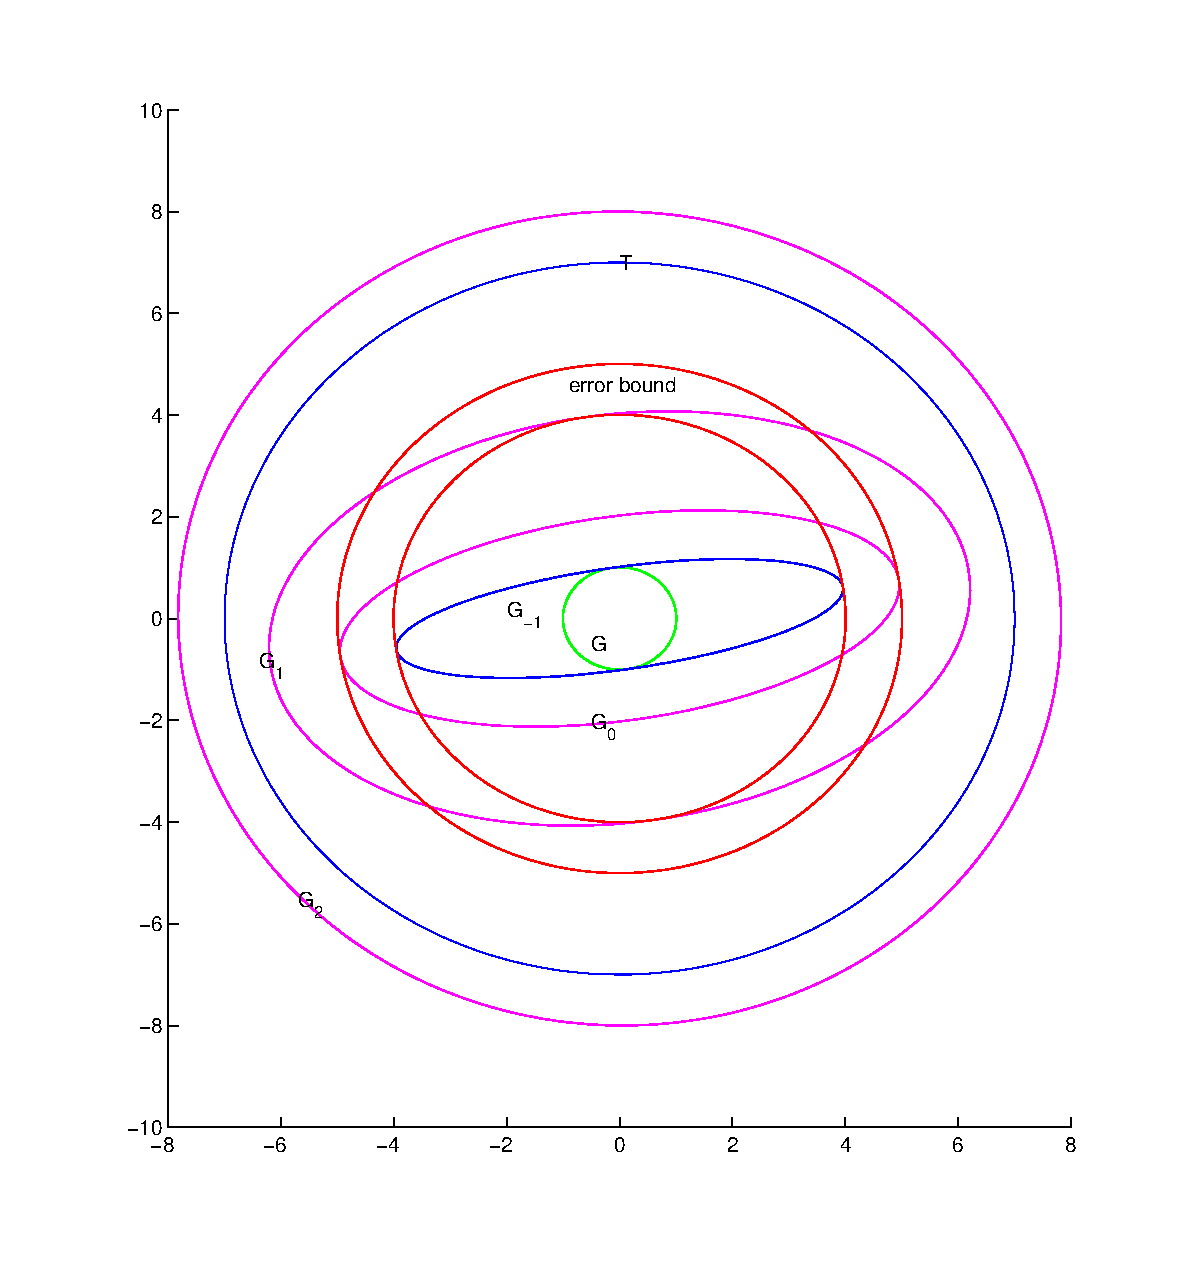
\includegraphics[width = 0.8\textwidth, height = 0.5\textheight]{sys.eps}
%\end{center}
%\caption{Иллюстрация взаимного расположения множеств ошибок в $\mathbb{R}^2$.}
%\label{krasn}
%\end{multicols}
%\end{figure}
\end{remark}

\subsection{Неравенства концентрации для сумм случайных величин ---  неравенства Чернова, Хевдинга, Бернштейна, Азумы}
\end{comment}

%По мотивам лекции Голубева, обзора Лугоши.

%\begin{enumerate}
%\item
\begin{problem}[Неравенство  Чернова]

Доказать, что неравенство Чернова для неотрицательной случайной величины $X$
\begin{equation*}
\mathbf{P}\{ X >t\}\leq \inf_{s>0}\mathbf{E}\exp(sX-st)
\end{equation*}
 дает более завышенную границу по сравнению с моментной границей
\begin{equation*}
\mathbf{P}\{ X >t\}\leq \min_{q>0}\mathbf{E}[X^q]t^{-q},
\end{equation*}
 то есть 
\begin{equation*}
\min_q\mathbf{E}[X^q]t^{-q}\leq \inf_{s>0}\mathbf{E}\big[\text{e}^{s(X-t)}\bigl]
\end{equation*}
\end{problem}

\begin{remark} Использовать следствие из неравенства Маркова: для монотонной возрастающей неотрицаиельной функции $\phi(\cdot)$ и произвольной неотрицательной случайной величины $X$ верно
\begin{equation*}
\mathbf{P}\{\phi(X)\geq \phi(t)\}\leq \frac{\mathbf{E}\phi(X)}{\phi(X)}.
\end{equation*}
\end{remark}

%\item 
%\begin{problem}[Неравенство Чернова для суммы случайных величин]

%\end{problem}

%\item
\begin{comment}
\begin{problem}
Пусть $\xi_t$ ~--- гауссовские случайные величины с нулевым средним и $\mathbf{E}\xi_t^2 = \sigma^2_t\leq\sigma$. Тогда 
\begin{equation*}
\mathbf{E}\max_{t\in T}\xi_t \leq \sqrt{2\sigma^2\log(n)},
\end{equation*}
здесь $n = \#T$~--- число элементов $T$.
\end{problem}
\begin{remark}
Основная идея доказательства: если случайные величины $\xi'_t>0$ имеют тяжелые хвосты, то 
\begin{equation*}
\max_{t\in T} \xi'_t \asymp \sum_{t\in T}\xi'_t.
\end{equation*}

Для любого $\lambda>0$ 
\begin{equation*}
\max_{t\in T} \xi_t = \lambda^{-1}\log\big[\max_{t\in T} \rm e^{\lambda \xi_t}\bigr]\leq \lambda^{-1}\log\big[\sum_{t\in T}\rm e^{\lambda \xi_t}\bigr].
\end{equation*}
Воспользоваться далее неравенством Йенсена и получить
\begin{equation*}
\begin{split}
\mathbf{E}\max_{t\in T} \xi_t \leq \frac{\log(n)}{\lambda} + \frac{\sigma^2\lambda}{2}.
\end{split}
\end{equation*}

Минимизировать по $\lambda$.

\end{remark}
\end{comment}

\begin{problem}[Лемма Хефдинга] Пусть $X$--- случайная величина, такая что $\mathbf{E}X =0$, $a\leq X\leq b$. Тогда для $s>0$ верно
\begin{equation*}
\mathbf{E}\exp(s X)\leq \exp\bigg[\frac{s^2(b-a)^2}{8}\biggr]
\end{equation*}
\end{problem}

\begin{remark}
Использовать выпуклость экспоненты, для $a\leq x\leq b$

\begin{equation*}
\text{e}^{sx} \leq \frac{x-a}{b-a} \text{e}^{sb}+\frac{b-x}{b-a}\text{e}^{sa} 
\end{equation*}

Получить 

\begin{equation*}
\mathbf{E}\text{e}^{sx} \leq \text{e}^{\phi(u)}
\end{equation*}

где $u = s(b-a)$, $\phi(u) = -pu+\log(1-p+p\text{e}^u)$, $p = -a/(b-a)$.
Найти $\phi^{\prime\prime}(u)$,   $\phi(0)$, $\phi^{\prime}(0)$.

Показать, что 
\begin{equation*}
\phi^{\prime\prime}(u)\leq \frac{1}{4}.
\end{equation*}

Используя формулу Тейлора, получить  
\begin{equation*}
\phi(u) \leq \frac{u^2}{8}\leq \frac{s^2(b-a)^2}{8}.
\end{equation*}
\end{remark}

\begin{problem}[Теорема Хефдинга] Пусть $\xi_t$, $t\in T$ ~--- независимые случайные величины, такие что $\xi_t\in[a,b]$. Тогда
\begin{equation*}
\mathbf{P}\bigg\{\bigg|\frac{1}{n}\sum_{t\in T}\big(\xi_t-\mathbf{E}\xi_t\bigr)\biggr|\geq x\biggr\}\leq 2\exp\bigg\{-\frac{2nx^2}{(b-a)^2}\biggr\}.
\end{equation*}
\end{problem}
\begin{remark}
Ввести случайную величину $\xi = \frac{1}{n}\sum_{i=1}^n(\xi_i-\mathbf{E}\xi_i)$.
Воспользоваться неравеством Чернова и леммой Хевдинга для $\xi$, чтобы получить
\begin{equation*}
\mathbf{P}\{\xi>x\}\leq \exp\bigg\{\min_{\lambda}\bigg[-\lambda x + \frac{\lambda^2}{8}\frac{(b-a)^2}{n}\biggr]\biggr\}.
\end{equation*}
Затем найти оптимальное $\lambda$.  Аналогичное неравенство справедливо для $-\xi$.
\end{remark}

\begin{problem}[Неравенство Беннетта]
Пусть $X_1,\dots, X_n$ независимые центрированные ограниченные случайные величины, такие, что с вероятностью $1$ выполнено $|X_i|\leq c$.
Пусть $\sigma^2 = \sum_{i=1}^n\text{Var}\{X_i\}$.
 Тогда для любого $t>0$ 
\begin{equation*}
\mathbf{P}\bigg\{\sum_{i=1}^n X_i>t\biggr\}\leq \exp\bigg(-\frac{n\sigma^2}{c^2}h\bigg(\frac{ct}{n\sigma^2}\biggr)\biggr),
\end{equation*}
где $h(u) = (1+u)\log(1+u)-u$ для $u\geq 0$.
\end{problem}
\begin{remark}
Введем $\sigma_i^2 = \mathbf{E}[X_i^r]$ и $F_i = \sum_{r=2}^{\infty}\frac{s^{r-2}\mathbf{E}[X_i^r]}{r!\sigma_i^2}$.
Используя разложение для ряда Тейлора $\exp(sX)$, показать, что 
\begin{equation*}
\mathbf{E}[e^{sX_i}]\leq \exp(s^2\sigma^2_iF_i).
\end{equation*}

Из ограниченности  $X_i$ получить оценку
\begin{equation*}
F_i\leq \frac{\exp(sc)-1-sc}{(sc)^2}.
\end{equation*} 
Далее воспользоваться неравенством Чернова для $X_i$ и минимизировать правую часть в неравенстве Чернова по $s$.
\end{remark}

\begin{problem}[Неравенство Бернштейна]
При выполнении условий предыдущей теоремы для любого  $\epsilon>0$ верно 
\begin{equation*}
\mathbf{P}\bigg\{\frac{1}{n}\sum_{i=1}^n X_i>\epsilon\biggr\}\leq \exp\bigg(-\frac{n\epsilon^2}{2\sigma^2+2c\epsilon/3}\biggr).
\end{equation*}
\end{problem}

\begin{remark} 
Показать, что верно элементарное неравенство 
\begin{equation*}
h(u)\geq \frac{u^2}{2+2u/3}
\end{equation*}
и использовать неравенство Беннетта.

Отметим, что в случае $\sigma^2<< \epsilon$ оценка принимает вид, аналогичный  неравенству больших уклонений (см. следующую задачу).
\end{remark}
%\end{enumerate}
\begin{comment}
\begin{problem} Пусть $Y$ случайная величина,  $Y\in [-1,+1]$ и $\mathbf{E}[Y]=0$. Тогда для любого $t\geq 0$ верно 
\begin{equation*}
\mathbf{E}[\exp(tY)]\leq \exp(t^2/2).
\end{equation*}
\end{problem}

\begin{remark}
Использовать выпуклость $\exp(tx)$, а именно для $x\in[-1,1]$ верно.
\begin{equation*}
\text{e}^{tx}\leq \frac{1}{2}(1+x)\text{e}^{t} +\frac{1}{2}(1-x)\text{e}^{-t}
\end{equation*}
Подсчитать оценку математического ожидания $\mathbf{E}[\text{e}^{tY}]$ используя разложение экспоненты в ряд Тейлора и элементарный факт $(2n)!>2^nn!$.  
\end{remark}

\begin{problem}[Мартингальное неравенство Азумы-Хевдинга]

Пусть $\{X_i\}_{i=0}^{\infty}$ мартингал по отношению к фильтрации $\{\mathcal{F}_i\}$, пусть $Y_i = X_i-X_{i-1}$ соответствующая последовательность приращений. Тогда, если существуют такие $c_i>0$, что $|Y_i|\leq c_i$ для всех $i$, то 
\begin{equation*}
\mathbf{P}\{\sup_{n\geq m} |X_n-X_0|\geq t\}\leq 2\exp\bigg\{\frac{-t^2}{2\sum_{i=1}^{m}c^2_i}\biggl\}
\end{equation*}
\end{problem}

\begin{remark}

\begin{enumerate}
\item \textit{Использовать теорему Дуба.} 
%\textbf{TODO}
\item \textit{Cпособ для доказательства не равномерного варианта теоремы использует результат задачи 12.}

Показать, что 
\begin{equation*}
\mathbf{E}\exp(sY_1+\dots+ sY_m) = \mathbf{E}\big[\exp(sY_1+\dots+sY_{m-1})\mathbf{E}[\exp(sY_m)|\mathcal{F}_{m-1}]\bigl] 
\end{equation*}
записать неравенство Чернова

\begin{equation*}
\mathbf{P}[Y_1+\dots+Y_m>t]\leq \exp\big[-st+\sum_{i=1}^mc^2_i s^2/2\bigr].
\end{equation*}
Остается оценить $s$ из минимизации правой части.
\end{enumerate}

\end{remark}

\end{comment}

%\begin{problem}
%Что можно сказать о том, как соотносятся между собой неравенство Бернштейна и Хевдинга? Рассмотреть неравенство Бернштейна в случаях, когда $\sigma^2>\epsilon$ и когда $\sigma^2<\epsilon$. Что можно сказать про достижимость неравенства Бернштейна? 
%\begin{remark}
%Рассмотреть предельную теорему Пуассона.
%\end{remark}
%\end{problem}

\begin{comment}
\subsection{Неравенства концентрации меры для функционалов от случайных величин.}
\medskip

\begin{problem}[Неравенство Эфрона-Стейна]
Пусть $X'_1,\dots,X'_n$ ~--- независимые копии $X_1,\dots,X_n$ и 
\begin{equation*}
Z'_i = g(X_1,\dots, X'_i,\dots,X_n).
\end{equation*}
Тогда верно неравенство 
\begin{equation*}
\text{Var}(Z)\leq \frac{1}{2}\sum_{i=1}^{n}\mathbf{E}[(Z-Z'_i)^2].
\end{equation*}
\end{problem}
\begin{remark}
 
Пусть $X_1,\dots, X_n$, произвольные независимые (не обязательно одинаково распределенные случайные величины) принимающие значения из $\mathcal{X}$ и пусть  $g: \mathcal{X}^n\to \mathbf{R}$ измеримая функция $n$ переменных. Показать, что для случайной величины $Z = g(X_1,\dots,X_n)$ верно 
\begin{equation*}
\text{Var}(Z) \leq \sum_{i=1}^n \mathbf{E}\big[ (Z-\mathbf{E}_iZ)^2\bigl],
\end{equation*}
где $\mathbf{E}_iZ = \mathbf{E}[Z|X_1,\dots,X_{i-1},X_{i+1},\dots,X_n]$.
\end{remark}
\begin{problem}[Случай функций с ограниченными  разностями]
Функция $g: \mathcal{X}^n\to \mathbf{R}$ является функцией с ограниченными разностями, если для некоторых $c_i,$  $1\leq i\leq n$.
\begin{equation*}
\sup_{x_1,\dots,x_n;\, x'_i\in\mathcal{X}} |g(x_1,\dots,x_n)-g(x_1,\dots,x_{i-1},x'_i,x_{i+1},\dots,x_{i+1},\dots,x_n)|\leq c_i. 
\end{equation*}
Выпишите неравенство Эфрона-Стейна для случая функций с ограниченными разностями.
\end{problem}
\medskip

\subsection{Вероятности больших уклонений}

\end{comment}
\begin{problem}
Для последовательности независимых одинаково распределенных величин $\xi_1,\xi_2,\dots$ с математическими ожиданиями $m = \mathbf{E} \xi_i$, дисперсиями $\text{Var} \xi_i = d$ и функцией распределения $F(x)$ верна следующая оценка вероятности больших отклонений $\mathbf{P}\Bigl\{\Bigl|\sum_{i=1}^n\xi_i -n m \Bigr|\geq n\epsilon \Bigr\}$: 

\begin{equation*}
\mathbf{P}\Bigl\{\Bigl|\sum_{i=1}^n \xi_i -n m \Bigr|\geq n\epsilon \Bigr\} \leq B_n(\phi(t_0))^n \exp\big(-t_0 n\epsilon \bigr) ,
\end{equation*}
где 
\begin{equation*}
\lim_{n\to\infty}B_n=\frac{1}{2},
\end{equation*}
\begin{equation*}
\phi(t)=\int_{-\infty}^{\infty}\text{e}^{t x}\,d F(x),
\end{equation*}
\begin{equation*}
m(t) = \frac{\phi^{\prime}(t)}{\phi(t)}.
\end{equation*}
%\begin{equation*}
%r(\lambda_0) = \text{e}^{-\lambda_0 c}R(\lambda_0),
%\end{equation*}
значение $t_0$ удовлетворяет условию  $m(t_0) = \epsilon$.
\end{problem}
\begin{remark}


Если использовать для оценки вероятности $\mathbf{P}\Bigl\{\Bigl|\sum_{i=1}^n\xi_i - n m\Bigr|\geq s\Bigr\}$ неравенство Чебышева, то при $s = \epsilon \sqrt{n}$ и $s=\epsilon n$, где $\epsilon$~--- некоторая постоянная, получается разный порядок сходимости вероятности. В отличае от первого случая, оценка при $s=\epsilon n$ является очень грубой. 

Доказательство существования, единственности, а также положительности $t_0$  может быть найдено в книге Кораллова Л.Б. и Я. Г. Синая <<Теория вероятностей. Случайные процессы>>. Воспользуемся методом Крамера вычисления асимптотики вероятностей. Покажите, что верно 
\begin{equation*}
\mathbf{P}\Bigl\{\Bigl|\sum_{i=1}^n \xi_i- n m\Bigr|\geq n \epsilon \Bigr\} \leq (R(t_0)\text{e}^{-t_0\epsilon})^n \idotsint\limits_{x_1+\dots+x_n>\epsilon n} \,dF_{t_0}(x_1),\dots,dF_{t_0}(x_n),
\end{equation*}
где $F_t(x) = \frac{1}{\phi(t)}\int_{-\infty}^{x} \text{e}^{t u}d F(u)$ ~--- функция распределения (проверьте).

Для того, чтобы оценить интеграл, рассмотрите случайные величины $\tilde{\xi}_1,\dots,\tilde{\xi}_n$ с распределением $F_{t_0}$, воспользуйтесь центральной предельной теоремой, чтобы показать, что $B_n\to1/2$ при ${n\to\infty}$.
\end{remark}

\begin{problem}
Сравнить оценки вероятности отклонения выборочного среднего от теоретического среднего для последовательности одинаково распределенных случайных величин $\xi_1,\dots,\xi_n$ с распределением Бернулли с вероятностью успеха $\lambda/n$, где $\lambda$ постоянна, получаемые с помощью неравенства Хевдинга, Бернштейна и неравенства больших уклонений из предыдущих задач.
\end{problem}
\medskip 

%Введем ряд обозначений
%\begin{equation*}
%\mathbf{P}_{n,c} = \mathbf{P}\biggl\{\Bigl|\sum_{i=1}^n\xi_i -\sum_{i=1}^m m_i\Bigr|%\geq cn\biggr\},
%\end{equation*}
%\begin{equation*}
%R(\lambda)=\int_{-\infty}^{\infty}\text{e}^{\lambda x}\,d F(x),
%\end{equation*}
%\begin{equation*}
%m(\lambda) = \frac{R^{\prime}(\lambda)}{R(\lambda)}.
%\end{equation*}

\begin{comment}
\medskip

Оказывается, что при условии 
\begin{equation}
R(\lambda)<\infty
\label{condition.R}
\end{equation}
верна более точная оценка 
\begin{equation*}
\lim_{n\to\infty}\frac{1}{n}\ln \mathbf{P}_{n,c} =\ln r(\lambda_0),
\end{equation*}

\medskip
Для того, чтобы это показать, докажите следующие утверждения.

\begin{problem}
Будем говорить, что $M^{+}$ есть верхний предел по вероятности случайной величины $\xi$, если $\mathbf{P}\{\xi>M^{+}\} = 0$ и $\mathbf{P}\{M^{+}-\epsilon\leq\xi\leq M^{+}\}>0$ для каждого  $\epsilon>0$. Нижний предел по вероятности можно определить тем же образом. Если $\mathbf{P}\{\xi>M\}>0$, ($\mathbf{P}\{\xi<M\}>0$) для всякого $M$, то $M^{+}=\infty$ ($M^{-}=-\infty$). Во всех остальных случаях $M^{+}$ и $M^{-}$ конечны.
Показать, что при условии \eqref{condition.R} 
функция $m(\lambda)$ имеет следующие пределы
\begin{equation*}
\lim_{\lambda\to\infty}m(\lambda) = M^{+},\quad \lim_{\lambda\to -\infty} = M^{-}.
\end{equation*}
\end{problem}
%\begin{remark}

%\textbf{TODO}

%\end{remark}

%\begin{remark}

%\textbf{TODO}

%\end{remark}
\begin{problem}
Для всякого $b>0$ существует такое $p(b,\lambda_0)>0$, что 
\begin{equation*}
\mathbf{P}_{n,c} \geq (R(\lambda_0)\text{e}^{-\lambda_0c})^n\text{e}^{-\lambda_0 b \sqrt{n}} p_n, 
\end{equation*}
причем $\lim_{n\to\infty}p_n = p(b,\lambda_0)$.
\end{problem}


\end{comment}
%\begin{remark}
%\textbf{TODO}
%\end{remark}
%\begin{problem}[Задача о среднем функции в смысле Леви --- про концентрацию меры на сфере вокруг медианного значения "хорошей" функции]
%\end{problem}
%\subsection{Изопериметрические неравенства Талаграна(?)}


\section{Геометрические вероятности}

\begin{problem}

Три бабочки капустницы садятся на круглый кочан капусты радиуса 1 случайным образом (имеется в виду, что место положение каждой бабочки -- с.в., равномерно распределенная на сфере) и независимо друг от друга. Если между двумя бабочками (геодезическое) расстояние оказывается меньше ${\pi \mathord{\left/ {\vphantom {\pi  2}} \right. \kern-\nulldelimiterspace} 2} $, то обе улетают. Найдите вероятность того, что на капусте сидят все три бабочки.

\end{problem}

\begin{problem}
Какова вероятность того, что $n$-угольник с вершинами, случайно расположенных на окружности, содержит ее центр?
\end{problem}

\begin{problem}
Найти среднюю длину секущих трехмерного куба с единичной длиной.
\end{problem}

\begin{problem}
Пусть в пространстве $\mathbb R^n$ с евклидовой нормой задан $n$-мерный шар единичного радиуса. Внутри него имеются две случайные точки с радиус-векторами ${\bf{r}}_1$ и ${\bf{r}}_2$ соответственно, имеющие равномерное пространственное распределение внутри шара. Найти распределение случайной величины, являющейся средним расстоянием между этими двумя точками $r = \left|{\bf r}_1 - {\bf r}_2\right|$.
\end{problem}

\begin{problem} (в 2х местах)
Пусть случайный вектор $X^{n} $ имеет равномерное распределение на единичной сфере в ${\mathbb R}^{n} $. Пусть $Y^{n} $ -- проекция $X^{n} $ на первую координатную ось. Докажите, что последовательность $\sqrt{n} Y^{n} $ сходится по распределению к стандартной нормальной случайной величине.

\begin{ordre} 
Показать сходимость по распределению нормы $X^{n} $ к единице. Воспользоваться соотношением
\[
P\{ \frac{\xi_1}{\xi_2} < x \} = \underset{t}{\int} P\{\xi_1 < xt \} f_{\xi_2}(t) dt
\] 
\end{ordre}
\end{problem}



\begin{problem}
Двое условились о встрече между $10$ и $11$ часами утра, причем договорились ждать друг друга не более $10$ минут. Считая, что 
момент прихода на встречу каждым выбирается <<наудачу>> в пределах указанного часа, найти вероятность того, что встреча состоится. 
\end{problem}


\begin{problem}
На плоскости проведены параллельные прямые на единичном расстоянии друг от друга, и на плоскость наугад бросается иголка длиной $L<1$. 
Угол между прямыми и иголкой и расстояние от середины иглы до ближайшей прямой являются независимыми с.в., равномерно распределенными 
на соответственно $(0,2\pi)$ и $(-1/2,1/2)$. С помощью серии таких опытов вычислить число $\pi$ с заданной точностью 
$\delta=1\%$ и с вероятностью ошибки не больше $\varepsilon=5\%$. 
\end{problem}

\begin{ordre}

Рассмотрим окружность диаметра $1$, т.е. длины $\pi$. Такая окружность с вероятностью $1$ пересекает дважды одну из прямых. 
Тогда, исходя из линейности математического ожидания числа попаданий иглы на прямую относительно длины иглы, для иглы длиной $L<1$ 
имеем ${\mathbb E}\xi_L = 2L/\pi$. 

\end{ordre}



\begin{problem}
Покажите, что средняя площадь ортогональной проекции куба с ребром единица на случайную плоскость равна $3/2$. 
\end{problem}

\begin{ordre}
Покажите, что  средняя площадь  ортогональной проекции всякого измеримого тела 
линейно зависит от площади его границы. 
Рассмотрим вспомогательное (см. предыдущую задачу) тело, у которого легко вычисляется средняя площадь ортогональной проекции. 
\end{ordre}

\begin{problem}
Рассмотрим звезды, находящиеся на расстоянии, не превышающем $R$ от наблюдателя. Для простоты будем считать, что все звезды имеют одинаковый диаметр $\delta$ и равномерное пространственное распределение с количеством звезд $\lambda$ на единицу объема. Показать, что при $R \rightarrow \infty$ любой участок неба будет полностью светящимся.   

\begin{remark}
В действительности такое явление не наблюдается. В связи с конечным возрастом вселенной ($14 \cdot 10^9$ лет) ее радиус ограничен величиной $ct$.
\end{remark}
\end{problem}

\begin{problem}
Пусть  $N$ точек независимо распределены в области $D$ n-мерного пространства, $P$ - вероятность того, что фигура $F$, образованная $N$ точками, обладает определенным свойством,
зависящим только от взаимного расположения точек. Область $D$ является измеримой по Лебегу и ее мара равна $V$. Обозначим как $P_1$ вероятность того, что $F$ обладает требуемым свойством для случайных точек в области $D_1 \supset D$. Докажите следующее соотношение для малых приращений $\delta V$:
 \[
 \delta P = N (P_1 - P) V^{-1} \delta V
 \]  

\end{problem}



\begin{problem}[Теорема Дворецкого]
Доказать, что для любого $\epsilon > 0$ и $k \in \mathbb{N}$
существует $N = N(k, \epsilon) < exp(C\frac{\log \epsilon}{\epsilon^2}k)$ такое, что любое конечномерное банахово пространство ($X, \Vert\cdot\Vert)$, где $\dim X > N$, содержит $k$-мерное подпространство $E$, являющееся $\epsilon$-евклидовым, т.е. в нем можно задать такую норму $\vert \cdot \vert$, что $\Vert x \Vert \leqslant \vert x \vert \leqslant (1 + \epsilon) \Vert x \Vert$ $\forall x \in E$.     

\end{problem}

\begin{problem}
Выберем наугад (равновероятно) $k$ вершин $m$-мерного куба $[0,1]^m$. Обозначим как $X$ выпуклую оболочку выбранных вершин. Пусть $p_{km}$ - вероятность того, что все вершины многогранника попарно смежны. Докажите справедливость следующей оценки при $m > 3$:

\[
p_{km} > 1 - \frac{k^4 \cdot 5^m}{4 \cdot 8^m}
\]
    
\end{problem}

\begin{problem}
На плоскости нарисована выпуклая фигура, ограниченная кривой длины $L$. Докажите, что ее диаметр, т.е. максимальное расстояние между двумя ее точками, не меньше $\frac{L}{\pi }$.
\end{problem}
\begin{ordre}
Проведите в случайном направлении прямую. Покажите, что 
математическое ожидание длины проекции фигуры на случайное направление равно 
$\frac{L}{\pi }$.
\end{ordre}

\begin{problem}
В московском метро можно провозить коробки, у которых сумма измерений (длины, ширины и высоты) не превосходит некоторой границы. Можно ли перехитрить правила, поместив одну коробку в другую (сумма измерений внутренней коробки больше суммы измерений внешней)?
\end{problem}
\begin{ordre}
Спроектируйте коробку на случайно выбранное (в пространстве) 
направление. Длина проекции коробки складывается из проекций отрезков, 
идущих по ее высоте, длине и ширине. Проекция внутренней коробки не 
превосходит проекции внешней.
\end{ordre}

\begin{problem}
Несамопересекающаяся кривая длины 22 находится внутри круга радиуса 1. Докажите, что найдется прямая, имеющая с этой кривой по крайней мере 8 общих точек.
Известно, что более половины поверхности Земли занимают океаны. Используя из географии только этот факт, докажите, что можно найти две диаметрально противоположные точки, обе попавшие в океан.
\end{problem}

\begin{problem}
На плоскости расположено $2n$ векторов, выходящих из начала координат и длиной не более 1. Доказать, что существует угол $\alpha$ такой, что при повороте каждого из векторов на угол $\pm \alpha$, их векторная сумма окажется не большей 1.  
\end{problem}


\section{Теория информации и кодирование}
\begin{comment}
\subsection{Основные определения}
Пусть $X$ - дискретная случайная величина, принимающая значения из конечного множества (алфавита) $A = \{a_1,..., a_{|A|}\}$. $P = \{\mathbb{P}\{X = a_i\} = p_{a_i}\}$ - вероятностное распределение $X$ на $A$.

\begin{definition} \textit{Словом} в алфавите $A$ будем называть реализацию последовательности случайных величин $X_1,...,X_n..$: $w = (x_1...x_n..)$, $x_i \in A$.
\end{definition}

\begin{definition} 
\textit{Энтропией} $H(X)$ случайной величины $X$ распределенной по закону $P$ называется:
\begin{center}
$H(X) = - \sum_{a \in A} p_a\log p_a$, где $\log = \log_2$.
\end{center}
Иногда вместо $H(X)$  используется запись $H(P)$.
Энтропия измеряется в битах и интерпретируется как мера неопределенности или информационного содержания случайной величины. Чем она больше, тем больше неопределенность. В качестве иллюстрации, читателю предлагается решить первую задачу.
\end{definition}
В случае нескольких случайных величин можно определить два тесно связанных понятия: \textit{условной энтропии} и \textit{совместной информации}.
\begin{definition}
\textit{Условной энтропией} двух с.в. $X$ и $Y$ называется $H(X|Y) = \sum_{a \in A} \mathbb{P}(Y = a)H(X|Y=a)$, где $H(X|Y=a) = \sum_{a' \in A} \frac{\mathbb{P}(X = a', Y = a)}{\mathbb{P}(Y = a)} \log \frac{\mathbb{P}(X = a', Y = a)}{\mathbb{P}(Y = a)}$. Условная энтропия характеризует ту среднюю степень неопределнности, содержащейся в $X$, если имеется некоторая информация об $Y$.
\end{definition}

\begin{definition}
\textit{Совместная информация} $I(X,Y) = H(X) - H(X|Y)$ определяет то, сколько информации об $X$ содержится в $Y$.
\end{definition}

\begin{definition}
\textit{Относительной энтропией} случайных величин $X \backsim P$ и $Y \backsim Q$ на множестве $A$ (или расстоянием Кульбака-Лейблера между ними) называется
\begin{center}
$KL(P||Q) = \sum_{a \in A} p_a \log \frac{p_a}{q_a}$. 
\end{center}
В статистике эта величина определяет то, насколько "неэффективно" использование распределения $Q$ для аппроксимации распределедния $P$, или как много дополнительных бит мы заплатим за такую аппроксимацию.
\end{definition}

\begin{definition}
\textit{Кодом} слова $w \in A^{len(w)}$ в алфавите $\Sigma$ называется отображение $C(w) : w \rightarrow \sigma$, $\sigma \in B^{len(\sigma)}$. $len(\sigma)$ - длина кодового слова.
\end{definition}

\subsection{Задачи}
\end{comment}
\begin{problem} \textit{Цена информации.} Имеется неизвестное число от $1$ до $n$, $n \geq 2$. Разрешается задавать любые вопросы с ответами ДА/НЕТ. При этом при ответе ДА игрок платит 1 рубль, а при ответе НЕТ - 2 рубля. Сколько необходимо и достаточно заплатить для отгадывания числа?
\end{problem}


\begin{problem}\textit{Задача о шляпах. Тодд Эберт (1998)}

Трех игроков отводят в комнату, где на них надевают (случайно и независимо) белые и черные шляпы. Каждый видит 
цвет других шляп и должен написать на бумажке одно из трех слов: <<белый>>, <<черный>>, <<пас>> 
(не советуясь с другими и не показывая им свою бумажку). Команда выигрывает, если хотя бы один из игроков назвал правильный 
цвет своей шляпы и ни один не назвал неправильного. Как им сговориться, чтобы увеличить шансы? 
Решите эту же задачу, если игроков $n=2^m -1$ $( m\in {\mathbb N} )$. 
\end{problem}

\begin{ordre}
Воспользуйтесь понятием кода Хемминга.
\end{ordre}

\begin{remark}
Докажем для случая трех игроков, что стратегий лучше (вероятность выигрыша больше  $ \frac{3}{4}$) не бывает. 

Единственная информация, которой владеет $i$-й игрок --- это цвета шляп двух других. Поэтому стратегия для $i$-го игрока должна зависеть 
только от этих двух цветов. В каждом случае имется три варианта ответа для игрока: $0$, $1$ или <<пас>>, т.е. всего $3^{12}$ различных 
стратегий. Поскольку есть $8$ вариантов расположения шляп на игроках, более выгодная стратегия должна обеспечивать выигрыш в $7$ вариантах. 
Тогда один из игроков должен угадать свой цвет в $3$ ситуациях. Значит, имеются для него ответы $\alpha_{i_1 j_1}$, 
$\alpha_{i_2 j_2}$, не являющиеся пасами. Но тогда в ситуациях $\overline{\alpha_{i_1 j_1}} i_1 j_1$ и 
$\overline{\alpha_{i_2 j_2}} i_2 j_2$ он ошибется, что противоречит предположению о $7$ выигрышных ситуациях. 

Таким образом, максимальная вероятность выигрыша равна $\frac{3}{4}$. 

\end{remark}




\begin{problem} \textit{Аксимоматиеское определение энтропии}.
Покажите, что приведенное выше определение энтропии естественным образом вытекает из следующих требований, накладываемых на величину, служащую количественной характеристикой меры неопределенности:
\begin{enumerate}
\item Значение функции $H(X)$ не меняется при перестановке чисел ${p_{a_1},..., p_{a_n}}$,
\item $H(X)$ непрерывная функция,
\item Выполняется равенство $H(p_1,...,p_n) = H(p_1 + p_2, p_3,..., p_n) + (p_1 + p_2) H(\frac{p_1}{p_1+p_2},\frac{p_2}{p_1+p_2} )$. То есть неопределенность в исходе опыта не зависит от того, осуществляется ли выбор среди всех возможных альтернатив одномоментно или в несколько этапов.
\end{enumerate}
\end{problem}

\begin{problem} 
\begin{enumerate}
\item Ф.М. Достоевский решил изменить своим привычкам и отправился на скачки. У него есть предворительные (априорные) данные о том, какие шансы на победу имеет каждая из восьми лошадей-участниц: $(\frac{1}{2}, \frac{1}{4}, \frac{1}{8}, \frac{1}{16}, \frac{1}{64}, \frac{1}{64}, \frac{1}{64}, \frac{1}{64})$. Оцените энтропию, которая содержится в такой информации. 
\item Сравните результат со случаем, когда все исходы равновероятны. Какое из двух респределений содержит больше информации?
\item Докажите в общем случае, что из всех дискретных распределений на дискретном множестве $A$, наибольшей энтропией обладает равномерное.
\end{enumerate}
\end{problem}

\begin{comment}
\begin{problem}
В таблице приведен прогноз погоды в г. Долгопрудный:
$p$ - вероятность наличия/отсутствия осадков, $q$ - вероятсноть того, что прогноз окажется верным.
\begin{table}[h]
\caption{Прогноз погоды}
\begin{center}
\begin{tabular}{|c|c|c|c|c|}
\hline
 &$p_{rain}$  &$p_{fine}$ & $q_{rain}$ & $q_{fine}$  \\
\hline
$15$ июня & $0.4$ & $0.6$ & $\frac{3}{5}$ & $\frac{4}{5}$\\
\hline
$15$ октября & $0.8$ & $0.2$ & $\frac{9}{10}$ & $\frac{1}{2}$\\
\hline
\end{tabular}
\end{center}
\end{table}
В какой из указанных двух дней прогноз дает нам больше информации о реальной погоде?
\begin{ordre}
\end{ordre}
\end{problem}

\begin{problem}
Пусть $\{X_i\}_{i=1}^n$ - независимые в совокупности одинаково распределенные случайные величины с распределением $P = \{p_{a_i}\}$. Доказать, что 
\begin{equation}
-\frac{1}{n} \sum_{i = 1}^n \log P(X_i) \rightarrow^{\mathbb{P}} H(X_1)
\end{equation}
Или, другими словами, $\forall \delta, \epsilon > 0 \exists n_0$ такое что $\forall n \geq n_0$:
\begin{equation}
\mathbb{P}(|-\frac{1}{n} \sum_{i = 1}^n \log P(X_i) - H(X_1)| < \delta) > 1-\epsilon.
\end{equation}

\begin{ordre}
Воспользутесь тем, что $-\mathbb{E} \log P(X) = H(X)$.
\end{ordre}
\end{problem}

\begin{remark} При достаточно больших значениях $n$ можно определить множество \textit{типичных последовательностей} или \textit{слов}, энтропия которых близка к истинной энтропии распределения $P$. Вероятность появления слова $w$
\begin{equation}
p_w = p_{x_1}...p_{x_n} = 2^{-n (-\frac{1}{n} \sum_{i = 1}^n \log P(X_i))}.
\end{equation}
\textit{Множеством $\delta$-типичных $n$-буквенных слов} назовем $T_{\delta}^{(n)}$:
\begin{equation}
T_{\delta}^{(n)} = \{w: 2^{-n(H(X) + \delta)} < p_w < 2^{-n(H(X) - \delta)} \}
\end{equation}
\end{remark}

\begin{problem} \textit{Асимптотическая равнораспределенность.}
Доказать, что:
\begin{enumerate}
\item Множество типичных слов ограничено: $|T_{\delta}^{(n)}| \leq 2^{n(H(X) + \delta)}$;
\item $|T_{\delta}^{(n)}| \geq (1-\epsilon)2^{n(H(X) + \delta})$ для достаточно больших $n$;
\item вероятность того, что $w$ - нетипично: $\mathbb{P}\{w \neq T_{\delta}^{(n)} \} \leq \epsilon$.
\end{enumerate}
\end{problem}

\begin{remark} Идея о типичных последовательностях лежит в основе кодирования. Например, $\delta$-типичные $n$-буквенные слова кодируются при помощи двоичных последовательностей длины $n(H(X) + \delta)$, нетипичные отбрасываются или представляются одним и тем же добавочным символом. Очевидно, что при декодировании (восстановлении) вероятность ошибки не превысит $\epsilon$.
\end{remark}

\begin{problem} Рассмотрите связь между доказательством принципа асимптотической равнораспределенности и эквивалентностью (для больших систем)энтропий Больцмана и Гиббса.
\end{problem}
\end{comment}

\begin{problem}
Пусть буква $X$ --- дискретная с.в., принимающая значения из алфавита $(x_1,\ldots,x_m)$ с вероятностями $(p_1,\ldots,p_m)$. 
Имеется случайный текст из $n$ букв $X$ (предполагается, что буквы в тексте независимы друг от друга). Общее количество таких 
текстов $2^{n\log m}$. Поэтому можно закодировать все эти слова, используя $n\log m$ бит. Однако, используя то обстоятельство, что 
$(p_1,\ldots,p_m)$ --- в общем случае неравномерное распределение, предложите лучший способ кодирования, основанный 
на усиленном законе больших чисел.
\end{problem}

\begin{ordre}
Пусть $\Omega=\{ \omega:\; \omega=(X_1,X_2,\ldots, X_n),\, X_i\in 1,2,\ldots,m\}$ --- пространство элементарных исходов. 
Вероятность появления слова $\omega=(X_1,X_2,\ldots, X_n)$ равна $p(\omega)=p_{X_1}\cdot\ldots\cdot p_{X_n}$. По теореме Колмогорова об 
у.з.б.ч. 
$$
-\frac{1}{n}\log p(\omega)=-\frac{1}{n}\sum\limits_{i=1}^{n}\log p_{X_i} \xrightarrow{\text{ п.н. }} 
-{\mathbb E}p(\omega)=-\sum\limits_{i=1}^{m}p_i\log p_i=H(p) 
$$
В частности, $\frac{S_n}{n}\xrightarrow{P}H(p)$, где $S_n=-\log p(\omega)=-\sum\limits_{i=1}^{n}\log p_{X_i}$. Это можно записать в виде 

$$
{\mathbb P}\Bigl( \Bigl| \frac{S_n-nH(p)}{n}\Bigr|>\delta \Bigr)  \xrightarrow{n\to\infty} 0 
$$
\end{ordre}

\begin{comment}
\begin{problem} \textit{Задача о пропускной способности канала с шумом.} Канал связи с шумом описывается матрицей переходных вероятностей $p(y|x)$, $x \in A$, $y \in B$. $A$ - входной алфавит, $B$ - выходной алфавит. Другими словами, $p(y|x)$ - вероятность принять $y$ при условии, что был послан символ $x$. \textit{Пропускной способностью} такого канала называется величина $C = \max_{\{p_x\}} I(x, y)$. $\{p_x\}$ множество всех возможных распределений на входном алфавите $A$.
Рассмотрим двоичный симметричный канал, $A =\{0, 1\}$, $B =\{0, 1\}$. Каждая из букв передается без ошибок с вероятностями $p$ и $1-p$ соответственно. Указать распределение, на котором достигается его максимальная пропускная способность.
\end{problem}
\begin{comment}
\begin{remark}
О связи совместная информации $I(x,y)$ и пропускной способности канала.  
\end{remark}

\begin{problem} \textit{Случайные коды.}
\end{problem}

\begin{problem} \textit{Оценка энтропии русского языка}
Рассмотрим алфавит $A$ состоящий из $34$х букв: $33$ буквы русского алфавита и пробел. На каждом шаге игроку необходимо угадать следующую букву текста, которая будет открыта, при условии, что он видит все буквы, открытые ранее. За каждую правильную догадку игрок получает $34$ рубля. Предложите стратегию, позволяющую оценить снизу энтропию русского языка.
\begin{ordre} Необходимо на каждом шаге выбирать ту букву, появление которой наиболее вероятно с учетом предыдущей информации. Тогда на шаге $n$ выигрыш может быть записан как $S_n = (34)^n \hat{p}(X_1...X_n)$, где $\hat{p}(X_1,...,X_n) = \sum_{a \in A} \hat{p}(a|x_{n-1}...x_1)$. Показать, что $\mathbb{E}\frac{1}{n}S_n \leq \log(34) + H(X)$, $H(X)$ - энтропия русского языка.
\end{ordre}   
\end{problem}
\begin{remark} Стоит ли писать что на этом подходе основывается построение кодов оптимальной длины?
\end{remark}

\end{comment}

\begin{problem}\textit{Неравенство Пинскера.} 
\textit{Расстоянием по вариации} между двумя распределениями называется $||\mathbb{P}_1 - \mathbb{P}_2||_1 = \sum_{a \in A} |\mathbb{P}_1(a) - \mathbb{P}_2(a)|$. Доказать, что между ним и расстоянием Кульбака-Лейблера справедливо следующее соотношение:\\
$KL(\mathbb{P}_1||\mathbb{P}_2) \geq \frac{1}{2\ln2} ||\mathbb{P}_1 - \mathbb{P}_2||_1^2$
\end{problem}

\begin{problem}
Рассмотрим две монетки: правильную ($Be(p = \frac{1}{2})$) и неправильную ($Be(q = \frac{1 +\epsilon}{2})$). Оценить минимальное число бросаний, необходимое для того, чтобы отличить первую от второй.
\end{problem}
\begin{comment}
\begin{remark} Необходимость построения нижних оценок возникает тогда, когда случайная последовательность генерируется одним из распределений $\{P_i\}$ (неизвестно каким), а наилучшая стратегия игрока зависит от вида истинного $P_k \in \{P_i\}$, о котором нет никакой информации  . 
\end{remark}
\end{comment}
\begin{problem}
Пусть казино делает $n$ бросаний, используя распределение вероятностей на бинарных словах длины $n$ $p\left(x\right)$, где $x=\left\{0,1\right\}^{n} $, известное игроку. При этом казино производит выплаты так, как если бы оно использовало распределении $q\left(x\right)$ (то есть выигранная ставка на 0, после выпадения $x$ исходов увеличивается в $\frac{q\left(x\right)}{q\left(x0\right)} $ раз, выигранная ставка на 1, после выпадения $x$ исходов увеличивается в $\frac{q\left(x\right)}{q\left(x1\right)} $ раз, см. семинар). Докажите, что у игрока есть стратегия, логарифм значения капитала которой равен расстоянию Кульбака-Лейблера $\sum _{x\in \left\{0,1\right\}^{n} }p\left(x\right)\log \frac{p\left(x\right)}{q\left(x\right)}  $ между распределениями $p$ и $q$.
\end{problem}

\begin{comment}
\begin{problem} \textit{Неравенство больших уклонений}
Рассмотрим последовательность незовисимых одинаково распределенных случайных величин $X_1, ..., X_n$, $X_i~Be(q)$. Доказать, что $-\frac{1}{n}\log \mathbb{P}(\frac{1}{n}\sum X_i \geq p) \rightarrow p\log \frac{p}{q} + (1-p)\log \frac{1-p}{1-q} = KL((p, 1-p)||(q, 1-q))$.
\begin{ordre}
\end{ordre}
\end{problem}

\begin{remark} 
Этот результат является следствием теоремы Санова, которая позволяет оценивать вероятности больших уклонений.. Приведем ниже её упрощенную формулировку.\\
\textit{Теорема Санова}
\end{remark}

\end{comment}



\section{Три кита математической статистики}

\section{Разные задачи}

\begin{problem}
Напомним, что сингулярными мерами называются меры, функции распределения $F(x)$ которых непрерывны, но точки их роста ($x$ -- точка роста $F(x)$, если для любого $\varepsilon >0$ выполняется: $F(x+\varepsilon )-F(x+\varepsilon )>0$) образуют множество нулевой меры Лебега. Покажите, что мера, соответствующая функции Кантора, сингулярна по отношению к мере Лебега.
\end{problem}


\begin{problem}
(Распределения канторовского типа).

Рассмотрим в $\sum _{k=1}^{\infty }2^{-k} X_{k}  $, где $X_{k} $ - взаимно независимые с.в., имеющие распределение Бернулли с параметром ${1\mathord{\left/ {\vphantom {1 2}} \right. \kern-\nulldelimiterspace} 2} $, сумму слагаемых с четными номерами, или, что с точностью до множителя 3 (в дальнейшем потребуется для удобства) есть $Y=3\sum _{s=1}^{\infty }4^{-s} X_{s}  $. Покажите, что функция распределения $F(x)=P\left\{Y\le x\right\}$ является сингулярной (когда не оговаривается относительно какой меры, подразумевается, что относительно меры Лебега).


\begin{ordre}
Можно рассматривать $Y$ как выигрыш игрока, который получает $3\cdot 4^{-k} $, когда $k$-е бросание симметричной монеты дает в результате решку. Ясно, что полный выигрыш лежит между 0 и $3\left(4^{-1} +4^{-2} +\ldots \right)=1$. Если первое подбрасывание монеты привело к решке, то полный выигрыш $\ge {3\mathord{\left/ {\vphantom {3 4}} \right. \kern-\nulldelimiterspace} 4} $, тогда как в противоположном случае $Y\le 3\left(4^{-2} +4^{-3} +\ldots \right)=4^{-1} $. То есть неравенство ${1\mathord{\left/ {\vphantom {1 4}} \right. \kern-\nulldelimiterspace} 4} <Y<{3\mathord{\left/ {\vphantom {3 4}} \right. \kern-\nulldelimiterspace} 4} $ не может быть осуществлено ни при каких обстоятельствах, значит $F(x)={1\mathord{\left/ {\vphantom {1 2}} \right. \kern-\nulldelimiterspace} 2} $ в интервале $x\in \left({1\mathord{\left/ {\vphantom {1 4}} \right. \kern-\nulldelimiterspace} 4} ,{3\mathord{\left/ {\vphantom {3 4}} \right. \kern-\nulldelimiterspace} 4} \right)$. Чтобы определить, как ведет себя функция распределения на интервале $x\in \left(0,{1\mathord{\left/ {\vphantom {1 4}} \right. \kern-\nulldelimiterspace} 4} \right)$, покажите, что на этом интервале график отличается только преобразованием подобия $F(x)={1\mathord{\left/ {\vphantom {1 2}} \right. \kern-\nulldelimiterspace} 2} F(4x)$.
\end{ordre}

\begin{remark}
Пример, когда свертка двух сингулярных распределений имеет непрерывную плотность: с.в. $X=\sum _{k=1}^{\infty }2^{-k} X_{k}  $ имеет равномерное распределение на $\left(0;1\right)$. Обозначим сумму членов ряда с четными и нечетными номерами через $U$ и $V$ соответственно. Ясно, что $U$ и $2V$ имеют одинаковое распределение и их распределение относится к канторовскому типу.
\end{remark}

\end{problem}

\begin{problem}
Доказать неравенство Чернова:

\[P\left\{\sum _{i=1}^{n}X_{i} >(p+t)n \right\}\le \exp \left\{nH\left(\left\{p+t,q-t\right\},\left\{p,q\right\}\right)\right\},\quad 0\le t\le q,\] 
где $X_{i} $, $i=1,...,n$ - независимые случайные величины, имеющие распределение Бернулли:
\[X_{i} =\left\{\begin{array}{cc} {1,} & {p,} \\ {0,} & {q=1-p;} \end{array}\right. \] 
$H\left(P,Q\right)=\sum _{j=1}^{m}-P_{j} \log \frac{P_{j} }{Q_{j} }  $ - относительное энтропийное «расстояние» между двумя (дискретными) распределениями вероятностей $P=\left(P_{1} ,\ldots ,P_{m} \right)$ и $Q=\left(Q_{1} ,\ldots ,Q_{m} \right)$ на пространстве элементарных исходов размера $m$.

\begin{ordre}
 
Воспользуйтесь техникой получения неравенства Азумы, рассказанной на лекции, а именно 

\noindent \textbf{а)} перейдите к положительной случайной величине $e^{\lambda \sum _{i=1}^{n}X_{i}  } $($\lambda >0$ - некий параметр). В теории вероятностей функция $\varphi _{Y} (\lambda )=E\left[e^{\lambda Y} \right]$называется производящей функции моментов случайной величины $Y$, так как при разложении в ряд Тейлора $\varphi _{Y} (\lambda )=E\left[e^{\lambda Y} \right]=E\left[\sum _{i=0}^{\infty }\frac{\lambda ^{i} }{i!} Y^{i}  \right]=\sum _{i=0}^{\infty }\frac{\lambda ^{i} }{i!} E\left[Y^{i} \right] $, где $E\left[Y^{i} \right]$ - \textit{i}-ый момент случайной величины $Y$.

\noindent \textbf{б)} применив неравенство Маркова , получите $P\left\{\sum _{i=1}^{n}X_{i} > \; m\right\}=P\left\{e^{\lambda \sum _{i=1}^{n}X_{i}  } >e^{m} \right\}\le \left(\frac{pe^{\lambda } +q}{e^{\lambda (p+t)} } \right)^{n} $ с параметризацией $m=(p+t)n$.

\noindent \textbf{в)} подобрав оптимальное значение ($\frac{pe^{\lambda } +q}{e^{\lambda (p+t)} } \to \mathop{\min }\limits_{\lambda } $), получите 

\[
P\left\{\sum _{i=1}^{n}X_{i} >(p+t)n \right\}\le \left(\left(\frac{p}{p+t} \right)^{p+t} \left(\frac{q}{q-t} \right)^{q-t} \right)^{n} 
\]
\[
= \exp \left\{n\left[-(p+t)\ln \frac{p+t}{p} -(q-t)\ln \frac{q-t}{q} \right]\right\}.
\] 


\end{ordre}

\begin{remark}
C точки зрения математической статистики 

\[
H\left(\left\{p+t,q-t\right\},\left\{p,q\right\}\right)=-(p+t)\ln \frac{p+t}{p} -(q-t)\ln \frac{q-t}{q} 
\]

-энтропийное расстояние между апостериорным (полученным после эксперимента) распределением $\left\{p+t,q-t\right\}$и априорным $\left\{p,q\right\}$. Таким образом, «граница» Чернова уменьшается экспоненциально с показателем равным n-кратному энтропийному расстоянию между апостериорным и априорным распределением вероятностей.\textbf{}

\noindent Более удобная запись «границы» Чернова:
\[P\left\{\sum _{i=1}^{n}X_{i} >(p+t)n \right\}\le \exp \left\{-\frac{2t^{2} }{n} \right\},\] 
так как для функции $f(t)=(p+t)\ln \frac{p+t}{p} +(q-t)\ln \frac{q-t}{q} $ имеем $f(0)=f'(0)=0$, $f''(t)=\frac{1}{(p+t)(q-t)} \ge 4$ для любого $0\le t\le q$, значит разложение Тейлора 
\[f(t)=f(0)+f'(0)t+f''(\xi )\frac{t^{2} }{2!} \ge 2t^{2} ,\quad 0<\xi <t.\]

\end{remark}

\end{problem}

\begin{problem}

Доказать оценку для больших уклонений в Бернуллиевской модели:
\[X_{i} =\left\{\begin{array}{cc} {1,} & {p,} \\ {0,} & {q=1-p;} \end{array}\right. \] 
$P\left\{\sum _{i=1}^{n}X_{i} =\left[\alpha n\right] \right\}\sim \frac{1}{\sqrt{2\pi \alpha (1-\alpha )} } \exp \left\{nH(\{ p,1-p\} ,\{ \alpha ,1-\alpha \} )\right\}$, $0<\alpha <1$ и $\alpha \ne p$

\noindent Как и в предыдущем домашнем задании для оценки Чернова: $H\left(P,Q\right)=\sum _{j=1}^{m}-P_{j} \log \frac{P_{j} }{Q_{j} }  $ - относительное энтропийное «расстояние» между двумя (дискретными) распределениями вероятностей $P=\left(P_{1} ,\ldots ,P_{m} \right)$ и $Q=\left(Q_{1} ,\ldots ,Q_{m} \right)$ на пространстве элементарных исходов размера $m$.

\begin{ordre}

Напомним, что производящей функцией (п.ф.) некоторой целочисленной неотрицательной случайной величины (с.в.) $\xi $ называется $\varphi _{\xi } (z)=Ez^{\xi } =\sum _{j=0}^{\infty }P\left\{\xi =j\right\} z^{j} $. Зная распределение с.в. можно получить ее п.ф., и наоборот, задание п.ф. однозначно определяет ее распределение: (для этого можно воспользоваться теорией функций комплексного переменного -- теоремой Коши -- для определения коэффициентов в разложении аналитической функции в ряд Лорана) $P\left\{\xi =k\right\}=\left[z^{k} \right]\varphi _{\xi } (z)=\frac{1}{2\pi i} \oint _{\left|z\right|=1}\frac{\varphi _{\xi } (z)}{z^{k+1} } dz $. Также следует напомнить, что п.ф. для суммы независимых с.в. справедливо $\varphi _{\sum _{i=1}^{n}X_{i}  } (z)=Ez^{\sum _{i=1}^{n}X_{i}  } =E\left[\prod _{i=1}^{n}z^{X_{i} }  \right]=\prod _{i=1}^{n}Ez^{X_{i} }  =\prod _{i=1}^{n}\varphi _{X_{i} } (z) $. Таким образом, в данной задаче $P\left\{\sum _{i=1}^{n}X_{i} =\left[\alpha n\right] \right\}=\left[z^{\left[\alpha n\right]} \right]\varphi _{\sum _{i=1}^{n}X_{i}  } (z)=\frac{1}{2\pi i} \oint _{\left|z\right|=\rho }\frac{\left(pz+q\right)^{n} }{z^{\left[\alpha n\right]+1} } dz $,\textbf{ }последний интеграл можно оценить с помощью методе перевала: перейдя к полярным координатам $z=\rho e^{i\theta } $ и сделав замену, получим:\textbf{}
\[\frac{1}{2\pi i} \oint _{\left|z\right|=1}\frac{\left(pz+q\right)^{n} }{z^{\left[\alpha n\right]+1} } dz =\frac{1}{2\pi } \int _{-\pi }^{\pi }e^{nf\left(\rho e^{i\theta } \right)} d\theta  ,\] 
где $f(z)=\ln \left(pz+q\right)-\left(\alpha -\frac{\varepsilon _{n} }{n} \right)\ln z$ ($\left[\alpha n\right]=\alpha n-\varepsilon _{n} $). Далее, нужно найти седловую точку и ограничиться интегрированием по её малой окрестности, разлагая подынтегральное выражение в ряд Тейлора.

\end{ordre}

\end{problem} % разное

\newpage


\renewcommand\refname{Литература}
% В самом списке 1. вместо [1]
\makeatletter
\renewcommand{\@biblabel}[1]{#1.}
\makeatother

\begin{thebibliography} {20}

\bibitem{1} 
Боровков А.А. Теория вероятностей. – М.: Наука, 1986.  (и более поздние издания)

\bibitem{2} 
Гнеденко Б.В. Курс теории вероятностей. – М: Наука, 1988. (и более поздние издания)

\bibitem{3}
Колмогоров А.Н. Основные понятия теории вероятностей. – М.: Наука. 1974. 

\bibitem{21}
Ширяев А.Н. Вероятность 1, 2 – М.: МЦНМО, 2011.


\bibitem{5} 
Натан А.А., Горбачев О.Г., Гуз С.А. Теория вероятностей: Учеб. пособие. – М.: МЗ Пресс – МФТИ, 2007. 

\bibitem{6} 
Розанов Ю.А. Лекции по теории вероятностей. - Долгопрудный: Издательский дом “Интеллект”, 2008. 

\bibitem{7} 
Коралов Л.Б., Синай Я.Г. Теория вероятностей. Случайные процессы. М.: МЦНМО, 2013.

\bibitem{4} 
Кельберт М.Я., Сухов Ю.М. Вероятность и статистика в примерах и задачах. Том. 1 Основные понятия теории вероятностей и математической статистики. М. МЦНМО, 2007.


\bibitem{8} 
Гмурман В.Е. Руководство к решению задач по теории вероятностей и математической статистике. – М.: Высшая школа, 1979. – 400 с. (и более поздние издания)

\bibitem{22}
Ширяев А.Н. Задачи по теории вероятностей. – М.: МЦНМО, 2011. 


\bibitem{9} 
Зубков А.М., Севастьянов Б.А., Чистяков В.П. Сборник задач по теории вероятностей. – М.: Наука, 1989. 

\bibitem{10} 
Прохоров А.В., Ушаков В.Г., Ушаков Н.Г. Задачи по теории вероятностей. Основные понятия. Предельные теоремы. Случайные процессы. – М.: Наука, 1986. 


\bibitem{12} 
Секей Г. Парадоксы в теории вероятностей и математической статистике. – М.: РХД, 2003. 

\bibitem{13} 
Flajolet P., Sedgewick R. Analytic combinatorics. Cambridge University Press, 2008. 

\bibitem{14} 
Ledoux M. Concentration of measure phenomenon, Providence, RI, Amer. Math. Soc., 2001 (Math. Surveys Monogr. V. 89)

\bibitem{15} 
Алон Н., Спенсер Дж. Вероятностный метод. Бином, 2006.

\bibitem{16} 
Кендалл М., Моран П. Геометрические вероятности. М.: Наука, 1972.

\bibitem{17} 
Motwani R., Raghavan P. Randomized algorithms. Cambridge Univ. Press, 1995.

\bibitem{18} 
Cover T.M., Thomas J.A. Elements of Information theory. Wiley-Interscience, 2006. 

\bibitem{19} 
Durrett R. Probability: Theory and Examples. Cambridge Univ. Press, 2010.

\bibitem{20} 
Кац М. Вероятность и смежные вопросы в физике. М.: Мир, 1965.


\end{thebibliography}




\end{document}